\documentclass{JINST}
\usepackage{cite}
\usepackage{tablefootnote}
\newcommand{\li}{$^{9}$Li~}
\newcommand{\he}{$^{8}$He~}
\newcommand{\beEIGHT}{$^{8}$Be~}
\newcommand{\beNINE}{$^{9}$Be~}
\newcommand{\liEIGHT}{$^{8}$Li~}
\newcommand{\liSEVEN}{$^{7}$Li~}


\title{DCGenSpec: A nuclear physics-based Monte Carlo of the \li  and \he 
comsogenic production in liquid scintillator experiments.}

\author{First Author$^a$, Second Author$^b$\thanks{Corresponding
author.}~ and Third Author$^b$\\
\llap{$^a$}Name of Institute,\\
  Address, Country\\
\llap{$^b$}Name of Institute,\\
  Address, Country\\
  E-mail: \email{CorrespondingAuthor@email.com}}


\abstract{Radioactive isotopes that decay into a $\beta$ and a delayed
  neutron a signficant background to liquid scintilator based neutrino
  experiments because this mimics the signature of low energy
  anti-neutrino scattering on free protons. Lithium-9 and Helium-8 are examples
of such isotopes. 
While estimating the absolute rate of production of theseisotopes poses a
challenge, the simulation of the decay spectrum 
is feasable.    This allows for template fits using the energy
distribution of backgrounds to
determine the normalization directly from the data.    In this work we
present a Monte Carlo simulations of the \li/\he decay spectra,
incorporating all of the  the published decay branches of these
isotopes.  The
generator presented here is generic code that can be interfaced to any
detector simulation.   As our example, we present results from the
generator interfaced to the simulations of the Double Chooz reactor experiment.}


\keywords{Keyword1; Keyword2; Keyword3}

\begin{document}

\section{Introduction}


      Many neutrino experiments have published results of cosmogenic background
measurements needed for
      the precise predictions of neutrino oscillations.   A good
      review is provided in Ref.~\cite{doi:10.1146/annurev.nucl.54.070103.181248}.     In
      general, backgrounds come from the cosmic ray muons themselves,
      fast neutrons produced by the cosmic rays, and also isotopes
      produced when the cosmic ray muons interact with the material in
      the detector.   The KamLAND experiment has published an extensive
comparison of
      cosmogenic background measurements with 
      predictions based on Monte Carlo simulations
      ~\cite{PhysRevC.81.025807} and shown that, overall, there is
      good agreement
      with the experimental measurements.
     
      For scintillator-based, low-energy antineutrino detectors, such
     as those used on reactor experiments, a particularly important
     class of backgrounds are nuclear decays that produce a $\beta$
     and a neutron.      These mimic the signature of the 
     ``Inverse Beta Decay'' (IBD) interaction:
      \mbox{$\bar{\nu}_e + p \rightarrow e^+ + n$}
      which are signal events in oscillation experiments.   
      The most 
      important cosmogenically produced background isotopes 
      in liquid scintillator are 
      \li and \he, which both decay to a $\beta^-$ and a neutron.  Current 
     detectors cannot distinguish a $\beta^-$-based background event
     from the $\beta^+$-based signal, despite the additional $\gamma$s
     from positron annihilation.    The lifetimes of these isotopes
     are long,  257 and 172 ms, respectively, and hence are difficult
     to efficiently veto.    And the endpoints of the $\beta$ spectra
     are 13.6 and 8.6 MeV, respectively, and so a large fraction of
     these decays populate the signal region of reactor experiments,
     which is typically less than $\sim$8 MeV.
      
     The absolute rate of \li and \he production is difficult to
     predict.  However,  the relative rate of production and also the
     energy spectra can be well-modeled.  Because the events extend to
     energies beyond the signal region, a template of these
     backgrounds can be fit in the $>$8 MeV range, and the
     normalization can be determined.   This is the method used in the
     Double Chooz experiment \cite{PhysRevLett.108.131801,PhysRevD.86.052008,PhysRevD.87.011102}.

     This paper reports on a generator for \li and \he spectra that
     can be used in reactor-based experiments.   We first provide a
     brief overview of the generator, and then present the results, in
     comparison with results from Double Chooz.  
      
`
\section{The Cosmogenics Generator Input and Outputs}
\label{section1}

 \begin{figure}[t]
  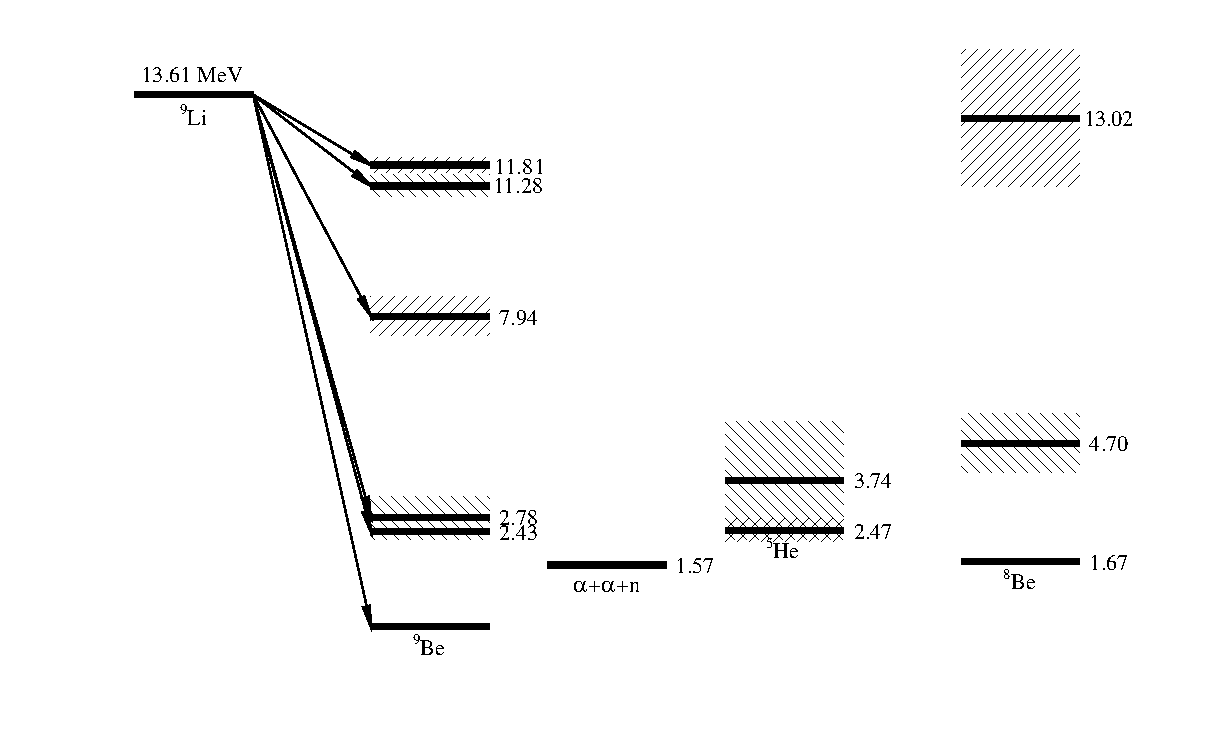
\includegraphics[scale=0.65]{Lithium9DecayScheme.eps}
  \label{DecayScheme}
  \caption{An energy level schematic of the \li decay scheme. }
 \end{figure}


 \begin{figure}[t]
 \begin{center}
  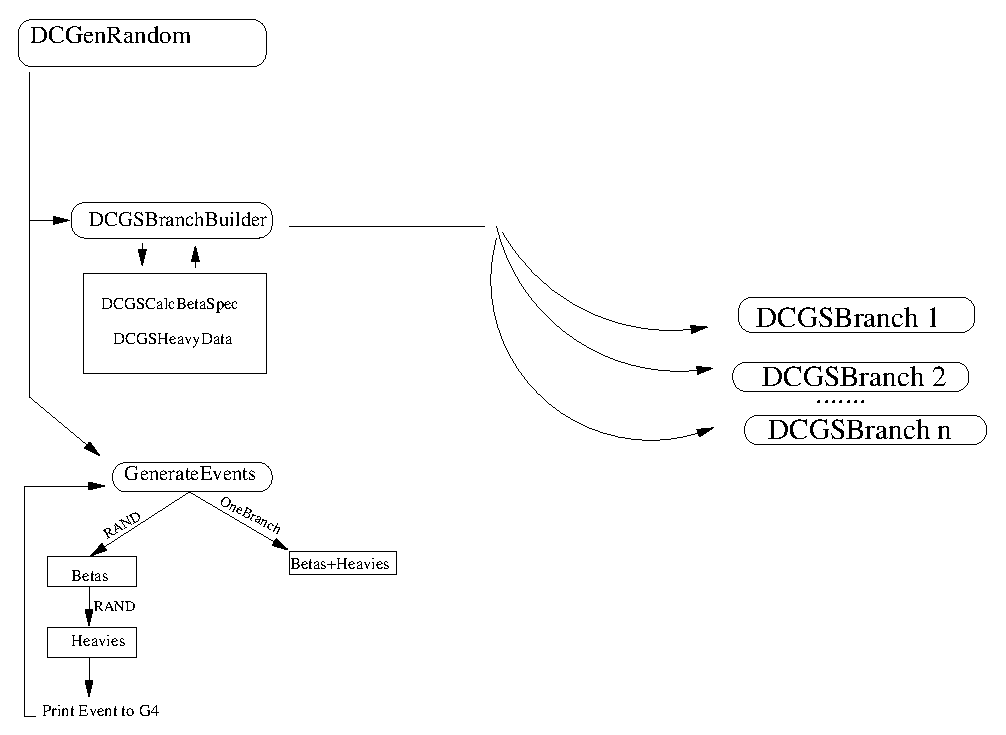
\includegraphics[scale=0.65]{tmp_xfig.eps}
  \label{OperDiagram}
  \caption{An operational diagram of the generator. }
    \end{center}
 \end{figure}

Figure ~\ref{DecayScheme} shows the different energy states of the different
isotopes the \li can decay to; mainly $^8$Be and $^5$He followed by the break up
into neutrons and alphas. The energy states for those isotopes are as indicated.
The decay widths (resonance parameters) associated with each of these states are
also represented by the hatched bands, which are drawn to scale. The generator
incorporates information on the branching ratios and their associated
uncertainties as well. We have done a literature review and decided to highlight some facts constructing the \beNINE states:
\begin{itemize}
 \item  Similar states, "Mirror Nuclei", share similar characterisitcs; an example is the decay of $^{9}$C to $^{5}$Li used 
 to understand the \beNINE decay to \heFIVE. As explained in ~\cite{PhysRevC.75.045803} a cluster model applicable to $^{9}$C could be used to deduce less-known
 states in \beNINE.
 \item A state that apparently not allowed by energy conservation could, in principle, be permissible 
 if the decay uncertainties are large.
 \item A parallelism can be drawn between the well-known \beNINE state (i.e. 11.81, 11.28) and the low-lying less known states 
 (i.e. 2.43,2.78,7.94) if the spins assigments are similar.
 \item When possible, the highest energy state (11.81 MeV) was chosen as a reference state since it is a well documented state ~\cite{Prezado200355}.
 \item The \heFIVE + $\alpha$ state becomes dominant for the higher energy decay of \beNINE states ~\cite{Descouv}. 
 \item The experimental detection difficulty of the low-lying states of \beNINE is because of the large width and overlapping nature of such states.
 
 
\end{itemize}


The states are presented in tables ~\ref{tabgs} to ~\ref{tab5}. We would also like to note the experimental interest in the \beNINE decay excited states stems from the fact that such states are important for three-body 
$ \alpha + \alpha +n $ reactions in astrophysics.

\subsection*{\it Beta-decay}

The generator starts by a beta decay into one of the energy states of the
\beNINE based on a conserved random probability ($b_{1} + b_{2} + .....= 1$) and
according to the branching ratios shown in table \ref{tab:betaStates}. The
branching ratios and the decay widths are extracted from ~\cite{Tilley2004155}. The beta
energies are calculated as the difference between the two energy states
incorporating the decay widths as Breit-Weigner distributions. The shape of the
emitted beta spectra is then calculated based on the well-known Fermi function.

\subsection*{\it Heavies}

The generator then proceeds to the decay of the \beNINE into either \beEIGHT or
\heFIVE through either neutron emission or alpha decay; respectively. The
momentum of
the final state particle is calculated according to 
a simplified momentum-splitting formula;

  \begin{equation}
K_1 =  \frac{m}{M} \Delta E
\end{equation}
and 
\begin{equation}
K_2 =  \frac{M-m}{M} \Delta E
\end{equation}
where $m$ is the mass of one of the daughters, $M$ is the decaying mass, ($K_1 , K_2$) are kinetic energies and
$\Delta E$ is the transferred energy. 

The decay into "Heavies" (neutrons or alphas) is also subject to widths of the
energy levels of the \heFIVE and \beEIGHT. The branching ratio ($BR$) of the
decays are ilustrated in table~\ref{tab2} to table~\ref{tab5} along with the energies of each
state,; each with its associated uncertainties. All the values were extracted
from the literature shown.

In the same spirit, we decided to investigate decay routes for the other important,
but less signficant, cosmogenic isotope \he \footnote{As published by KamLAND,\he is expected to be a $\sim$ 10\% contamination
to the \li, ~\cite{PhysRevC.81.025807}.}. In tables~\ref{tabHE} are the different decay
branches for the \he.






...
%the decay states of \li and \he, as presented in 
% in Table~\red{tab:states}.   The uncertainties associated with
%these are also taken into account {\bf what does this mean?}.  

 


\begin{table}[tb]
\caption{\label{tab:betaStates} {\bf Beta decay levels of the \li ground state. 
}: Excitation energies ($E$) and the widths ($\Gamma_E$); branching ratios
($BR$) and their associated uncertainties ($\delta BR $).~\cite{Tilley2004155}}
\begin{center}
\begin{small}
\begin{tabular}{l l l l }
\hline
%\multicolumn{5}{|c|}
\hline
\beNINE $E_x$ (MeV) & $\Gamma_E$ (KeV)& BR & $\delta$ BR   \\
\hline
1. 0 & $\pm$0.0& 0.492 & $\pm$0.009   \\ 
2. 2.43& $\pm$0.78 & 0.297 & $\pm$0.03   \\
3. 2.78  & $\pm$1080& 0.158 & $\pm$0.03   \\
4. 7.94 & $\pm$1000 & 0.015 & $\pm$0.005   \\
5. 11.28 & $\pm$575 & 0.011 & $\pm$0.002   \\
6. 11.81 & $\pm$400 & 0.027 & $\pm$0.002   \\
\hline
\hline
\end{tabular}
\end{small}
\end{center}
\end{table}



\begin{table}[tb]

\caption{\label{tabgs} {\bf \beNINE (g.s.) }: The ground state is stable as illustrated in this table.}

\begin{center}
\begin{small}
\begin{tabular}{l l l l l}
\hline
\hline
Sub-branch & BR & $\delta$ BR & $E$ (MeV) & $\Gamma_E$ (MeV) \\
\hline
1. $^{5}$He(g.s.) + $\alpha$ & 0.00 & $\pm$0.00 & 0.00 & $\pm$0.00 \\ 
2. $^{5}$He(1/2-) + $\alpha$ & 0.00 & $\pm$0.00 & 0.00 & $\pm$0.00 \\
3. $^{8}$Be(g.s.) + n & 0.00 & $\pm$0.00 & 0.00 & $\pm$0.00 \\
4. $^{8}$Be(2+) + n  & 0.00 & $\pm$0.00 & 0.00 & $\pm$0.00 \\
5. $^{8}$Be(4+) + n & 0.00 & $\pm$0.00  &  0.00 & $\pm$0.00 \\
\hline
\hline
\end{tabular}
\end{small}
\end{center}
\end{table}



%tablefootnote{
\begin{table}[tb]

\caption{\label{tab} {\bf \beNINE (2.43 MeV) }: Excitation energies ($E$)
and the widths ($\Gamma_E$); branching ratios ($BR$) and their associated
uncertainties ($\delta BR $), adapted from~\cite{PhysRevC.75.045803}.}

\begin{center}
\begin{small}
\begin{tabular}{l l l l l}
\hline
%\multicolumn{5}{|c|}
\hline
Sub-branch & BR & $\delta$ BR & $E$ (MeV) &
$\Gamma_E$ (MeV) \\
\hline
1. $^{5}$He(g.s.) + $\alpha$ & 0.025 & $\pm$0.025 & 2.467 & $\pm$0.648 \\ 
2. $^{8}$Be(g.s.) + n & 0.11 & $\pm$0.02 & 1.6654 & $\pm$0.00000557 \\
3. $^{8}$Be(2+) + n  & 0.865 & $\pm$0.045 & 4.695 & $\pm$1.513 \\
\hline
\hline
\end{tabular}
\end{small}
\end{center}
\end{table}



\begin{table}[tb]
\caption{\label{tab2} {\bf \beNINE (2.78 MeV)}: Excitation energies ($E$) and the widths ($\Gamma_E$); branching ratios ($BR$) and their associated uncertainties
($\delta BR $), adapted from~\cite{Prezado200543}.}
\begin{center}
\begin{small}
\begin{tabular}{l l l l l}
\hline
\hline
Sub-branch & BR & $\delta$ BR & $E$ (MeV) &
$\Gamma_E$ (MeV) \\
\hline
1. $^{5}$He(g.s.) + $\alpha$ & 0.25 & $\pm$0.25 & 2.467 & $\pm$0.648 \\ 
%2. $^{5}$He(1/2-) + $\alpha$ & 0.125 & $\pm$0.125 & 3.737 & $\pm$5.57 \\
3. $^{8}$Be(2+) + n & 0.75 & $\pm$0.75 & 1.6654 & $\pm$0.00000557 \\

\hline
\hline
\end{tabular}
\end{small}
\end{center}
\label{tab2}
\end{table}



\begin{table}[tb]
\caption{\label{tab3} {\bf \beNINE (7.94 MeV)}: Excitation energies ($E$) and the widths ($\Gamma_E$); branching ratios ($BR$) and their associated
uncertainties ($\delta BR $).}
\begin{center}
\begin{small}
\begin{tabular}{l l l l l}
\hline
\hline
Sub-branch & BR & $\delta$ BR & $E$ (MeV) &
$\Gamma_E$ (MeV) \\
\hline
1. $^{5}$He(g.s.) + $\alpha$ & 0.25 & $\pm$0.053 & 2.467 & $\pm$0.648 \\ 
2. $^{5}$He(1/2-) + $\alpha$ & 0.41 & $\pm$0.062 & 3.737 & $\pm$5.57 \\
3. $^{8}$Be(g.s.) + n & 0.018 & $\pm$0.009 & 1.6654 & $\pm$0.00000557 \\
4. $^{8}$Be(2+) + n  & 0.097 & $\pm$0.053 & 4.695 & $\pm$1.513 \\
\hline
\hline
\end{tabular}
\end{small}
\end{center}
\end{table}






\begin{table}[tb]
\caption{\label{tab4} {\bf \beNINE (11.28 MeV)}: Excitation energies ($E$)
and the widths ($\Gamma_E$); branching ratios ($BR$) and their associated
uncertainties ($\delta BR $), adapted from~\cite{PhysRevC.76.054605}.}
\begin{center}
\begin{small}
\begin{tabular}{l l l l l}
\hline
\hline
Sub-branch & BR\tablefootnote{Renormalized to one.} & $\delta$ BR & $E$ (MeV) & $\Gamma_E$ (MeV) \\
\hline
1. $^{5}$He(g.s.) + $\alpha$ & 0.76 & $\pm$0.30 & 2.467 & $\pm$0.648 \\ 
%2. $^{5}$He(1/2-) + $\alpha$ & 0.47 & $\pm$0.07 & 3.737 & $\pm$5.57 \\
3. $^{8}$Be(g.s.) + n & 0.03 & $\pm$0.01 & 1.6654 & $\pm$0.00000557 \\
4. $^{8}$Be(2+) + n  & 0.21 & $\pm$0.08 & 4.695 & $\pm$1.513 \\
%5. $^{8}$Be(4+) + n & 0.12 & $\pm$0.08  &  13.015 & $\pm$3.500 \\
\hline
\hline
\end{tabular}
\end{small}
\end{center}
\end{table}





\begin{table}[tb]
\label{tab5}
\caption{ {\bf  \beNINE (11.81 MeV)}: Excitation energies ($E$) and the widths
($\Gamma_E$); branching ratios ($BR$) and their associated uncertainties
($\delta BR $), adapted from~\cite{Prezado200355}.}
\begin{center}
\begin{small}
\begin{tabular}{l l l l l}
\hline
\hline
Sub-branch & BR & $\delta$ BR & $E$ (MeV) & $\Gamma_E$ (MeV) \\
\hline
1. $^{5}$He(g.s.) + $\alpha$ & 0.28 & $\pm$0.06 & 2.467 & $\pm$0.648 \\ 
2. $^{5}$He(1/2-) + $\alpha$ & 0.47 & $\pm$0.07 & 3.737 & $\pm$5.57 \\
3. $^{8}$Be(g.s.) + n & 0.02 & $\pm$0.01 & 1.6654 & $\pm$0.00000557 \\
4. $^{8}$Be(2+) + n  & 0.11 & $\pm$0.06 & 4.695 & $\pm$1.513 \\
5. $^{8}$Be(4+) + n & 0.12 & $\pm$0.08  &  13.015 & $\pm$3.500 \\
\hline
\hline
\end{tabular}
\end{small}
\end{center}
\end{table}





\begin{table}[tb]
\caption{\label{tab_he:betaStates} {\bf Beta decay levels of the \he ground state. 
}: symbols same as before for \li, ~\cite{Tilley2004155}}
\begin{center}
\begin{small}
\begin{tabular}{l l l l }
\hline
%\multicolumn{5}{|c|}
\hline
\liEIGHT $E_x$ (MeV) & $\Gamma_E$ (KeV)& BR & $\delta$ BR   \\
\hline
1. 0.981 & $\pm$0.0& 0.831 & $\pm$0.01   \\ 
2. 3.21& $\pm$1000.0 & 0.0256 & $\pm$0.0024   \\
3. 3.21  & $\pm$1000.0& 0.0544 & $\pm$0.0024   \\
4. 5.4 & $\pm$650.0 & 0.0256 & $\pm$0.0024   \\
5. 5.4 & $\pm$650.0 & 0.0544 & $\pm$0.0024   \\
6. 9.671?? & $\pm$1000.0 & 0.009 & $\pm$0.001   \\
\hline
\hline
\end{tabular}
\end{small}
\end{center}
\end{table}

\begin{table}[tb]
\caption{\label{tab_he_1} {\bf \liEIGHT (0.981 MeV)}: symbols are same as before.}
\begin{center}
\begin{small}
\begin{tabular}{l l l l l}
\hline
\hline
Sub-branch & BR & $\delta$ BR & $E$ (MeV) &
$\Gamma_E$ (MeV) \\
\hline
1. \liSEVEN + neutron & 0.00 & $\pm$0.0 & 0.00& $\pm$0.00 \\ 
\hline
\hline
\end{tabular}
\end{small}
\end{center}
\end{table}


\begin{table}[tb]
\caption{\label{tab_he_2} {\bf \liEIGHT (3.21 MeV)}: symbols are same as before.}
\begin{center}
\begin{small}
\begin{tabular}{l l l l l}
\hline
\hline
Sub-branch & BR & $\delta$ BR & $E$ (MeV) &
$\Gamma_E$ (MeV) \\
\hline
1. \liSEVEN & 1.00 & $\pm$0.00 & 2.511& $\pm$0.00 \\ 
\hline
\hline
\end{tabular}
\end{small}
\end{center}
\end{table}


\begin{table}[tb]
\caption{\label{tab_he_3} {\bf \liEIGHT (3.21 MeV)}: symbols are same as before.}
\begin{center}
\begin{small}
\begin{tabular}{l l l l l}
\hline
\hline
Sub-branch & BR & $\delta$ BR & $E$ (MeV) &
$\Gamma_E$ (MeV) \\
\hline
1. \liSEVEN & 1.00 & $\pm$0.00 & 2.0322& $\pm$0.00 \\ 
\hline
\hline
\end{tabular}
\end{small}
\end{center}
\end{table}

\begin{table}[tb]
\caption{\label{tab_he_3} {\bf \liEIGHT (3.21 MeV)}: symbols are same as before.}
\begin{center}
\begin{small}
\begin{tabular}{l l l l l}
\hline
\hline
Sub-branch & BR & $\delta$ BR & $E$ (MeV) &
$\Gamma_E$ (MeV) \\
\hline
1. \liSEVEN & 1.00 & $\pm$0.00 & 2.511& $\pm$0.00 \\ 
\hline
\hline
\end{tabular}
\end{small}
\end{center}
\end{table}


\begin{table}[tb]
\caption{\label{tab_he_4} {\bf \liEIGHT (3.21 MeV)}: symbols are same as before.}
\begin{center}
\begin{small}
\begin{tabular}{l l l l l}
\hline
\hline
Sub-branch & BR & $\delta$ BR & $E$ (MeV) &
$\Gamma_E$ (MeV) \\
\hline
1. \liSEVEN & 1.00 & $\pm$0.00 & 2.0322& $\pm$0.00 \\ 
\hline
\hline
\end{tabular}
\end{small}
\end{center}
\end{table}

\begin{table}[tb]
\caption{\label{tab_he_5} {\bf \liEIGHT (9.67??? MeV)}: symbols are same as before.}
\begin{center}
\begin{small}
\begin{tabular}{l l l l l}
\hline
\hline
Sub-branch & BR & $\delta$ BR & $E$ (MeV) &
$\Gamma_E$ (MeV) \\
\hline
1. $^{5}$He + n + t & 1.00 & $\pm$0.00 & 5.39& $\pm$0.60 \\ 
\hline
\hline
\end{tabular}
\end{small}
\end{center}
\end{table}


 \section{Results}
\label{section2} 
 In this section we present the results obtained with the generator,
 with and without incorporation into the Monte Carlo detector simulation used by
the Double Chooz
 collaboration.
The latter is based on 
 a GEANT4 (version) ~\cite{Geant4} simulation of the Double Chooz detector and the
generic liquid scintillator
 neutrino experiment package GLG4sim ~\cite{GLG4sim}. 
 
 
 
 The results obtained by running
the generator 
 independently of the Double Chooz detector simulations is refered to as
\textbf{{\emph{particle level}}}, while 
 results obtained by running the generator output through the simulations of the
Double Chooz detector 
 are refered to as  \textbf{{\emph{detector level}}}, ~\ref{PartDetDiagram}.
\subsection{Paricle Level}


\begin{figure}[t]
   \label{PartDetDiagram}	
 \begin{center}
  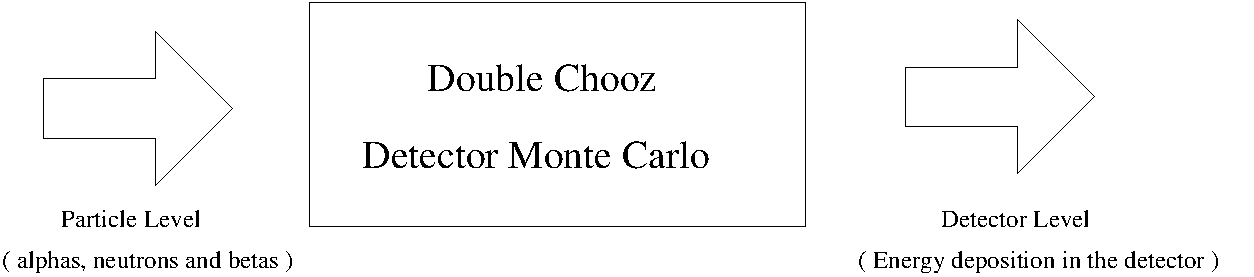
\includegraphics[scale=0.65]{Part_det_level.pdf}
  
    \end{center}
    \caption{An illustration of how the particle/detector level results fits into the grand scheme. }
 \end{figure}

%\begin{figure}
%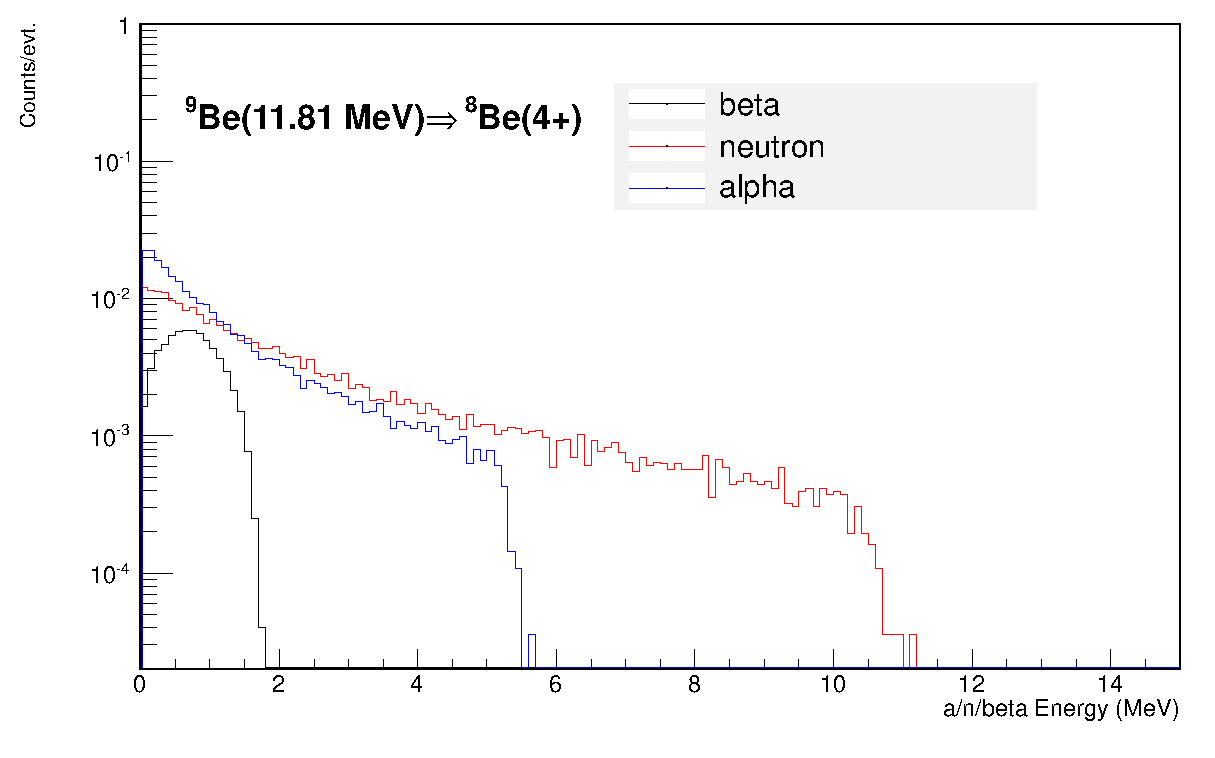
\includegraphics[scale=0.45]{a_n_beta_spect_c20.eps}
%\caption{
%Average target detector response evolution in time, as 
%measured by the mean energy of the Gd-capture peak arising from 
%interaction of spallation neutrons in the NT.
%\label{fig:gstability}}
%\end{figure}
%%%%%%%%%%%%%%%%%%%%%%%%%%%%%%%%%%%%%%%%%%%%
%%%%%%%%%%%%%%%%%%%%%%%%%%%%%%%%%%%%%%%%%%%%%
\begin{figure}[htp]
\label{Particle_level_energies}

  \centering
    
  \begin{tabular}{cc}

    % Requires \usepackage{graphicx}
    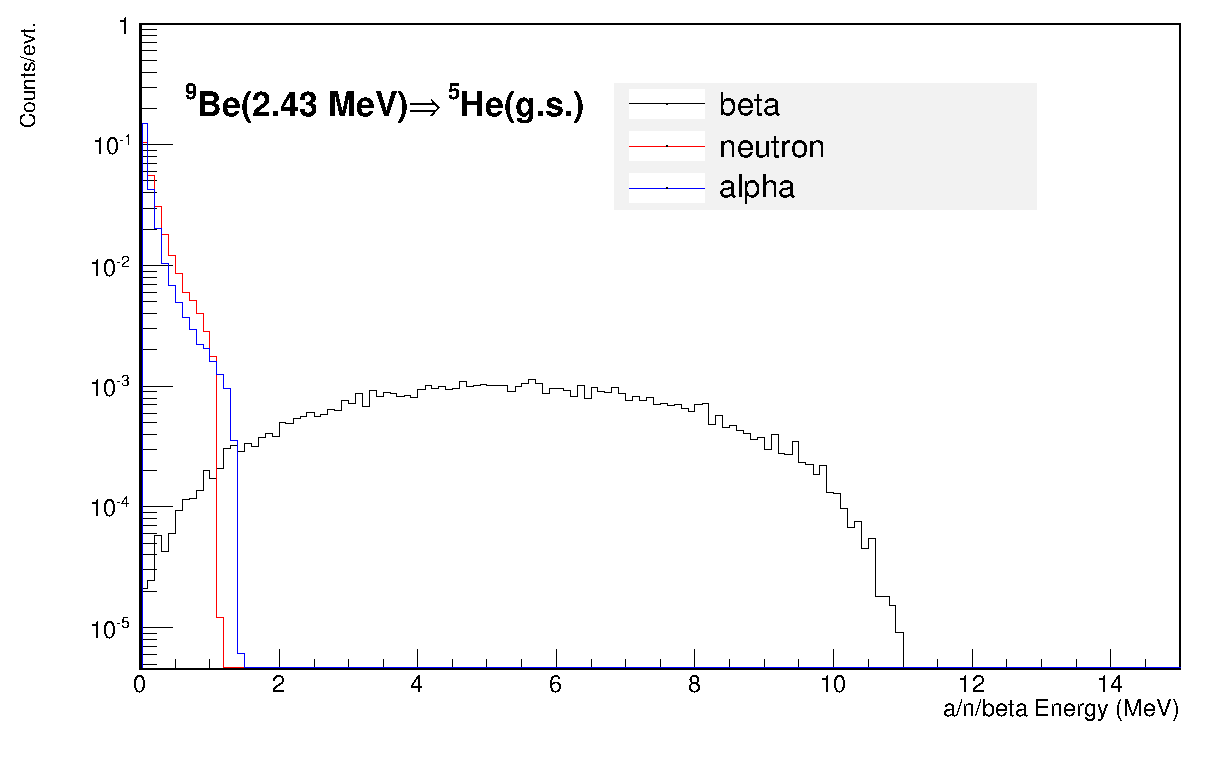
\includegraphics[width=70mm]{a_n_beta_spect_c1.eps} &
    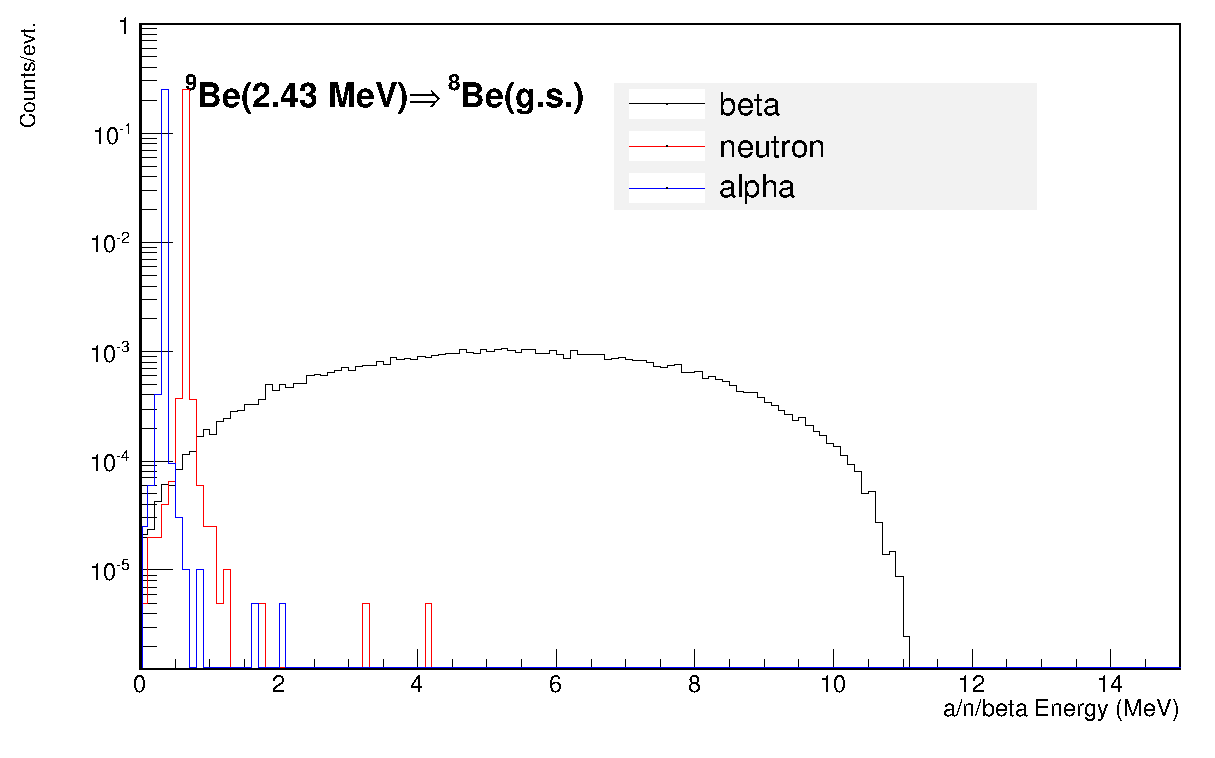
\includegraphics[width=70mm]{a_n_beta_spect_c2.eps} \\

    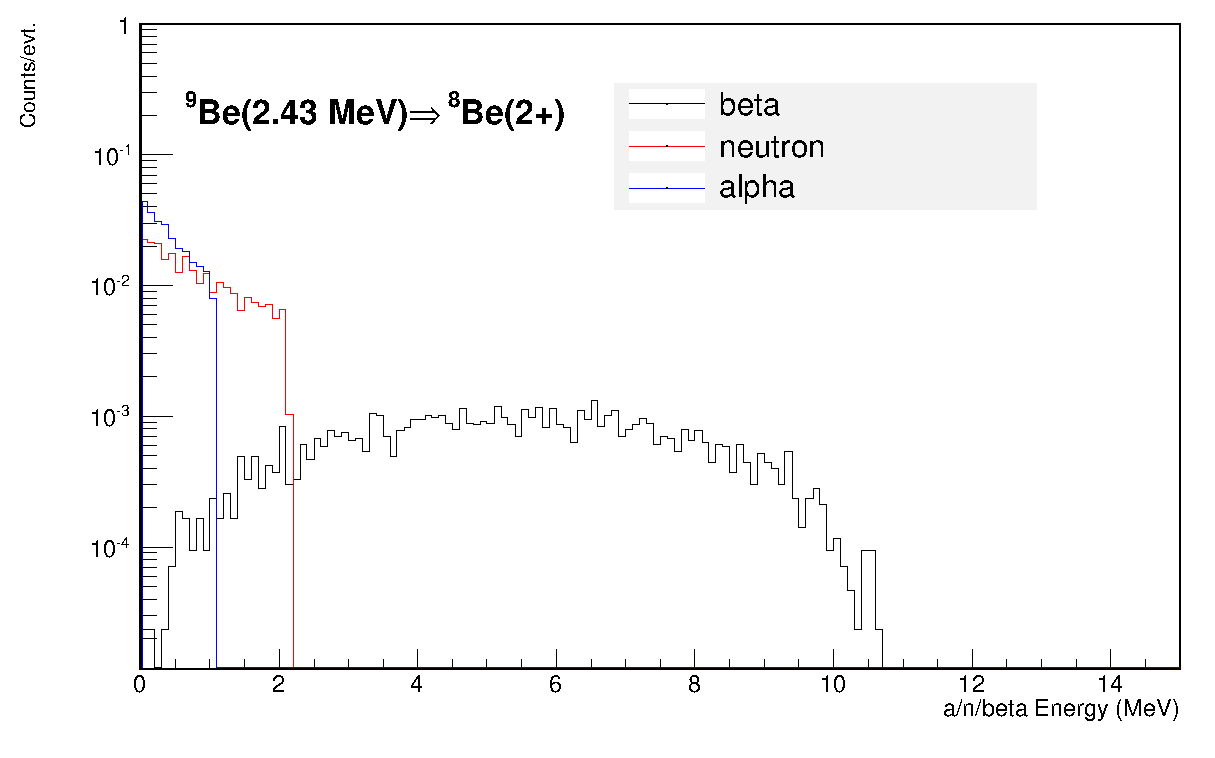
\includegraphics[width=70mm]{a_n_beta_spect_c3.eps}\\
    
   \end{tabular}
 \caption{Particle level energy distributions for the decay of the \beNINE 2.43 MeV state.}
    \end{figure}
%%%%%%%%%%%%%%%%%%%%%%%%%%%%%%%%%%%%%%%%%%%%%
%%%%%%%%%%%%%%%%%%%%%%%%%%%%%%%%%%%%%%%%%%%%%
    \begin{figure}[htp]
  \centering
      
  \begin{tabular}{cc}

    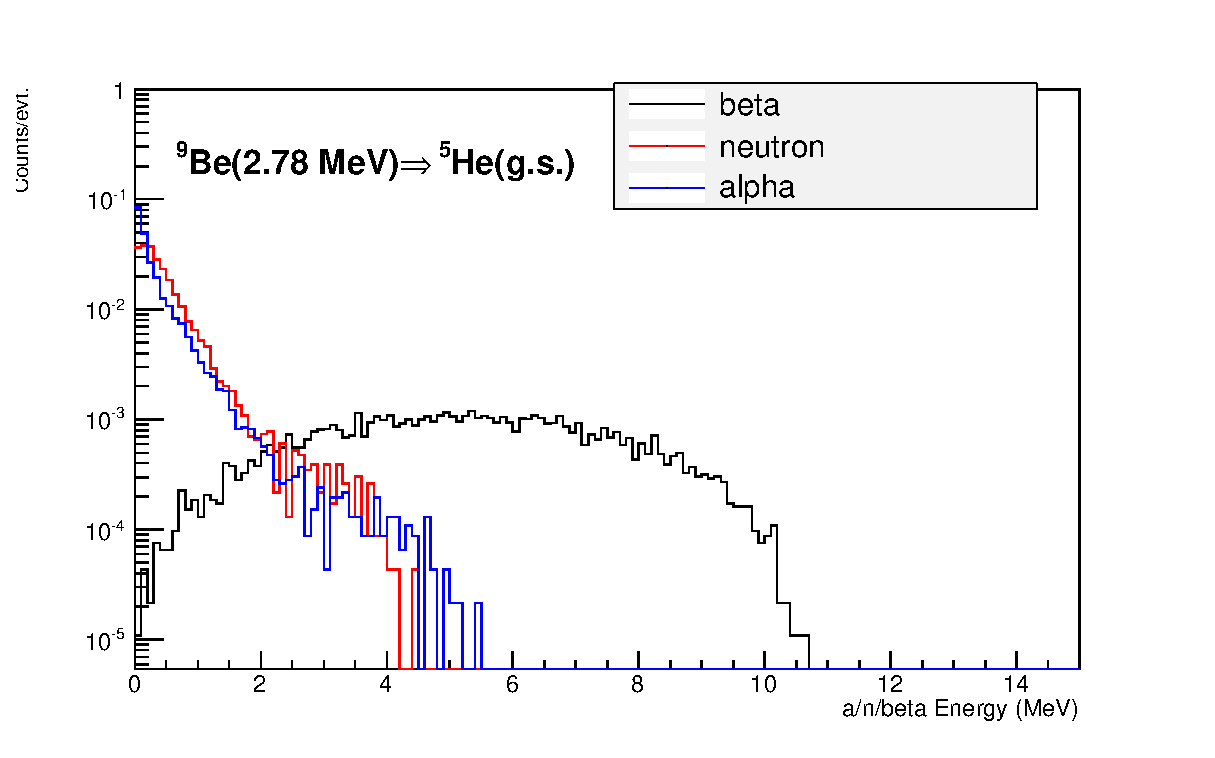
\includegraphics[width=70mm]{a_n_beta_spect_c4.eps}&

    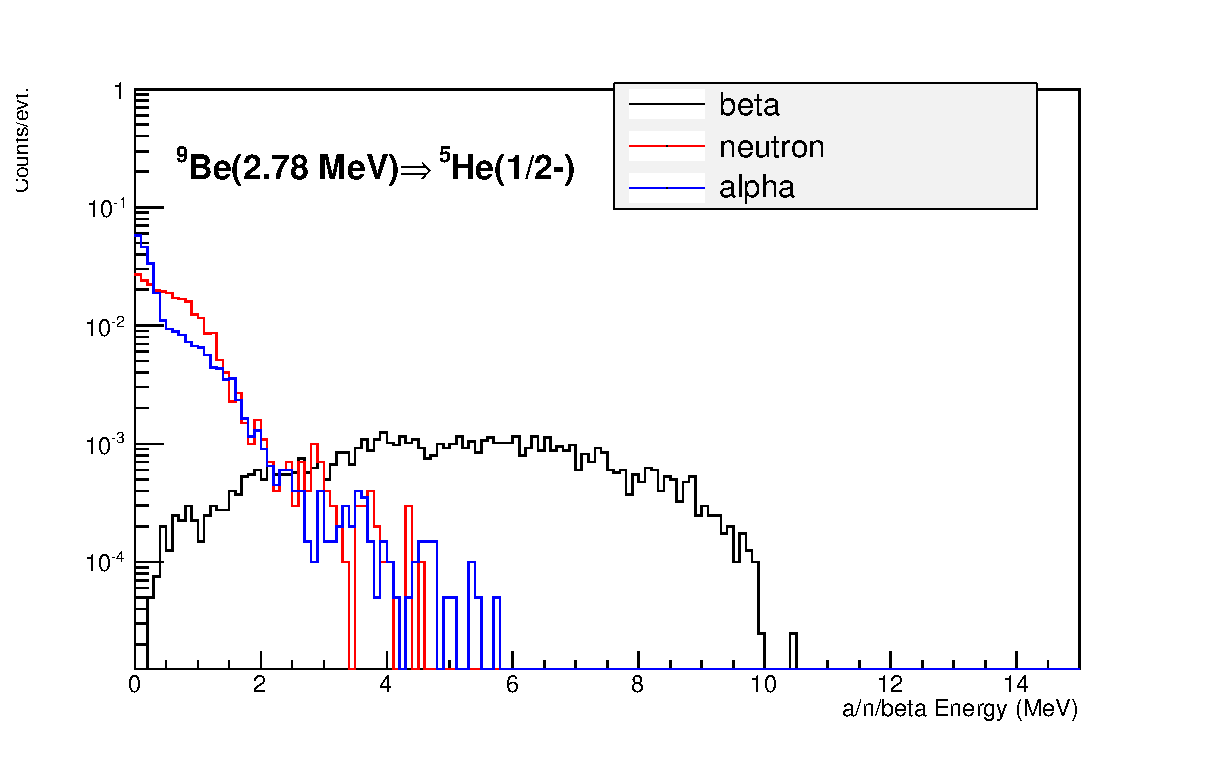
\includegraphics[width=70mm]{a_n_beta_spect_c5.eps}\\

      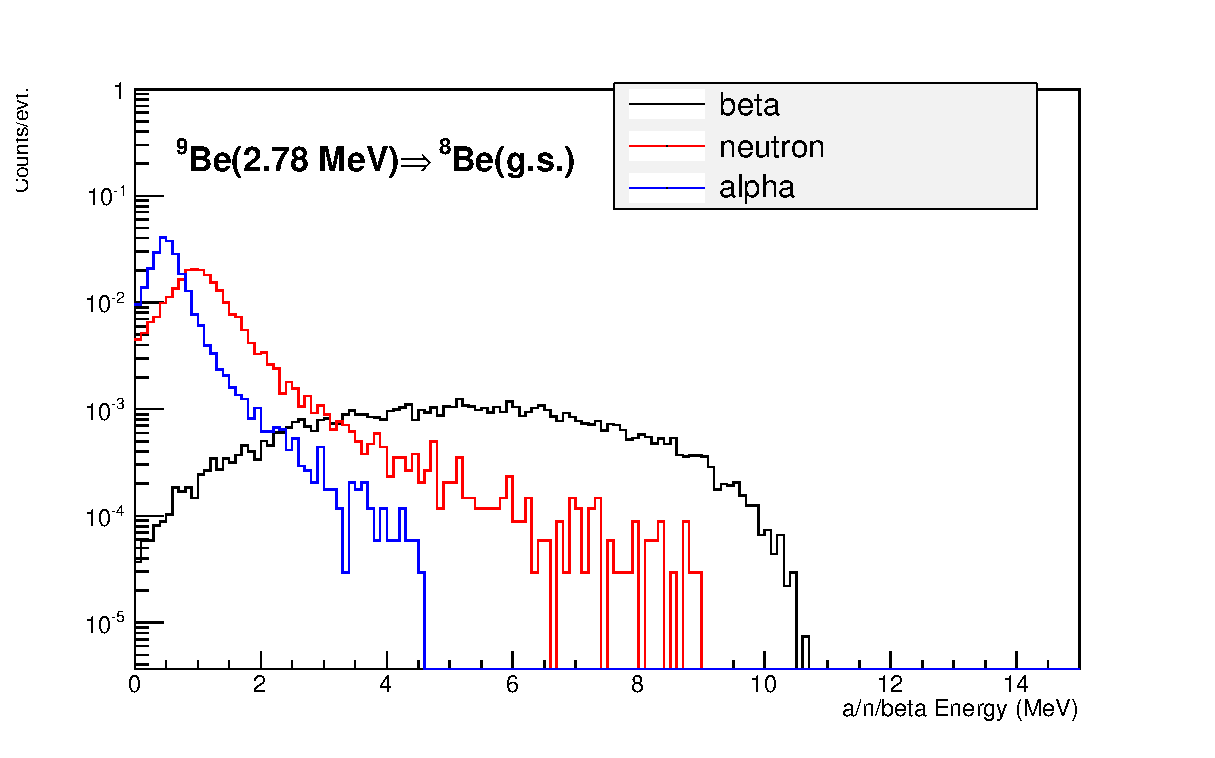
\includegraphics[width=70mm]{a_n_beta_spect_c6.eps}&
      
      
  \end{tabular}
  \caption{Particle level energy distributions for the decay of the \beNINE 2.78 MeV state.}
    \end{figure}

   %%%%%%%%%%%%%%%%%%%%%%%%%%%%%%%%%%%%%%%%%%%%%
%%%%%%%%%%%%%%%%%%%%%%%%%%%%%%%%%%%%%%%%%%%%% 
    \begin{figure}[htp]
     \centering
       
  \begin{tabular}{cc}

    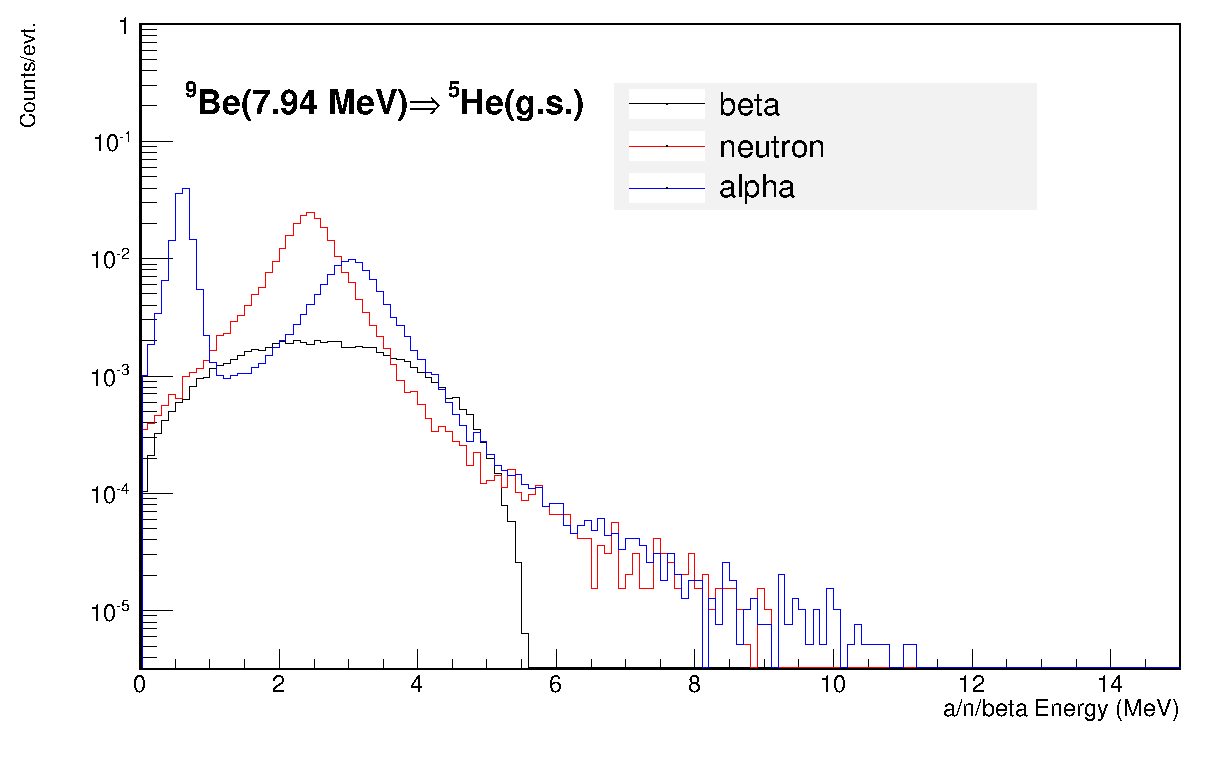
\includegraphics[width=70mm]{a_n_beta_spect_c7.eps} &
   
    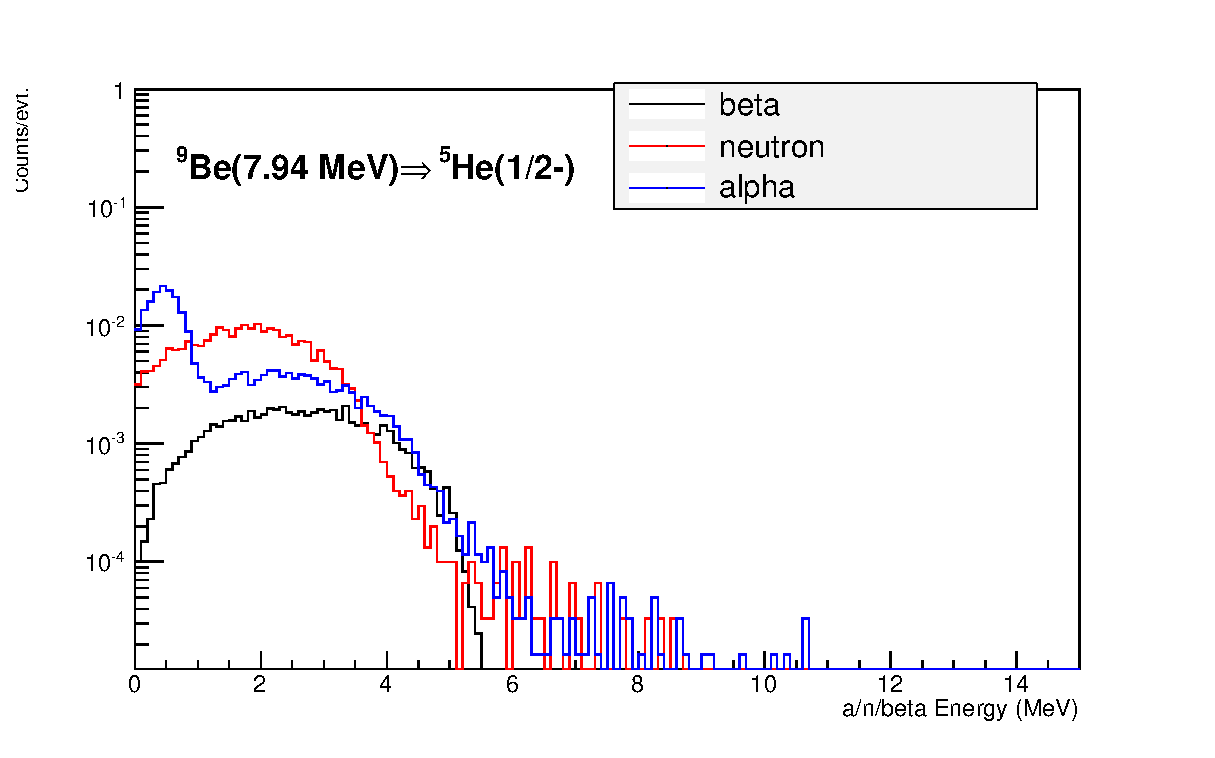
\includegraphics[width=70mm]{a_n_beta_spect_c8.eps} \\

    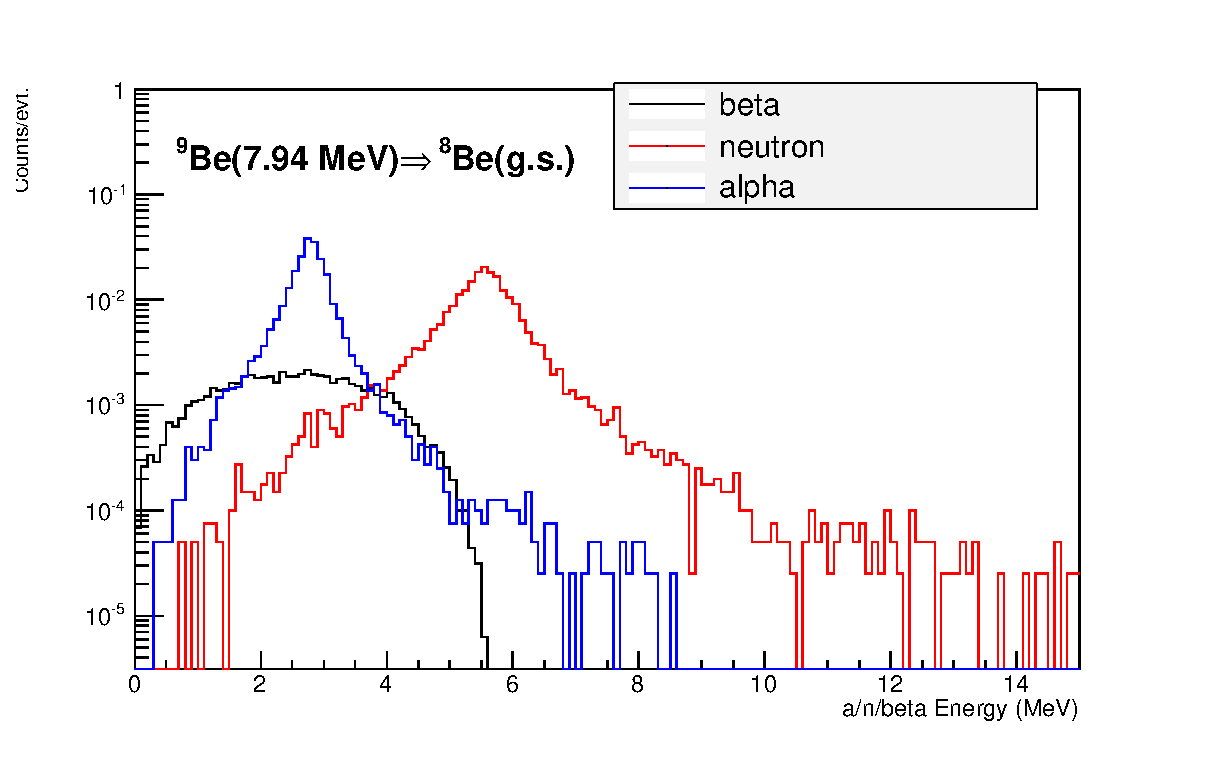
\includegraphics[width=70mm]{a_n_beta_spect_c9.eps} &
   
    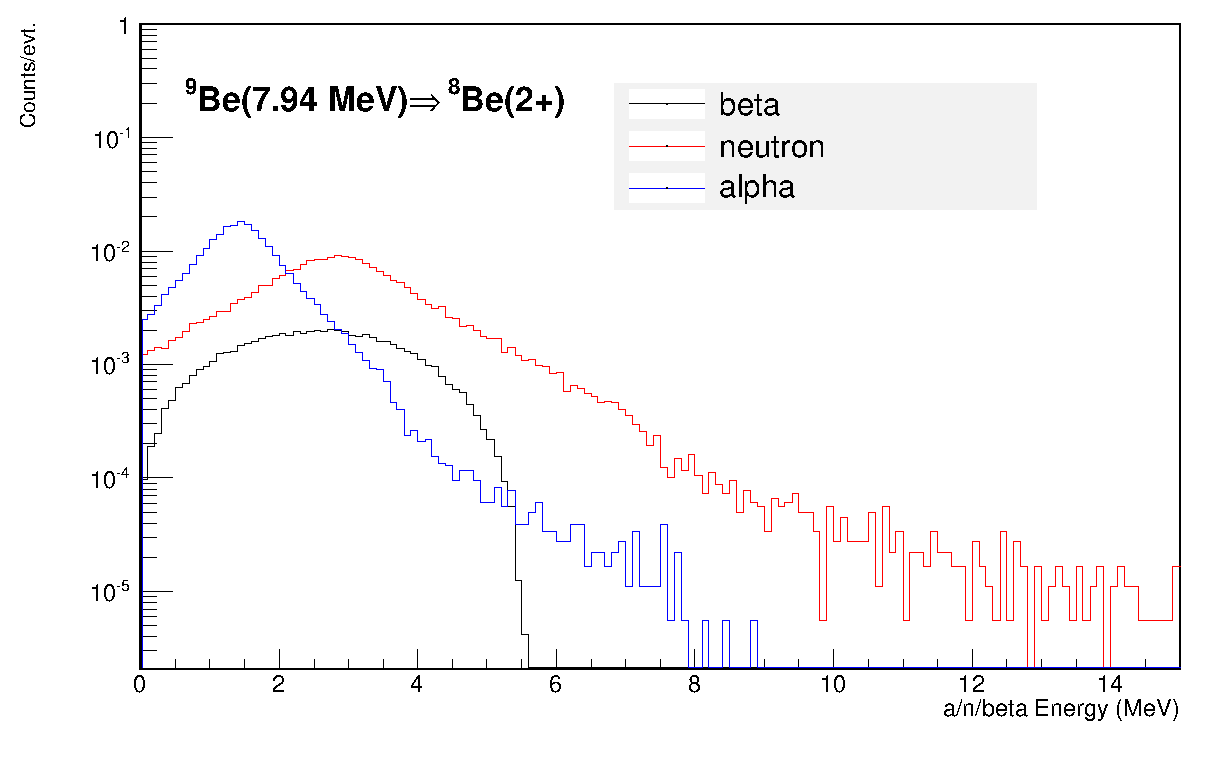
\includegraphics[width=70mm]{a_n_beta_spect_c10.eps}&

    
      \end{tabular}
  \caption{Particle level energy distributions for the decay of the \beNINE 7.94 MeV state.}
    \end{figure}

    %%%%%%%%%%%%%%%%%%%%%%%%%%%%%%%%%%%%%%%%%%%%%
%%%%%%%%%%%%%%%%%%%%%%%%%%%%%%%%%%%%%%%%%%%%%
    \begin{figure}[htp]
     \centering
     
  \begin{tabular}{cc}
    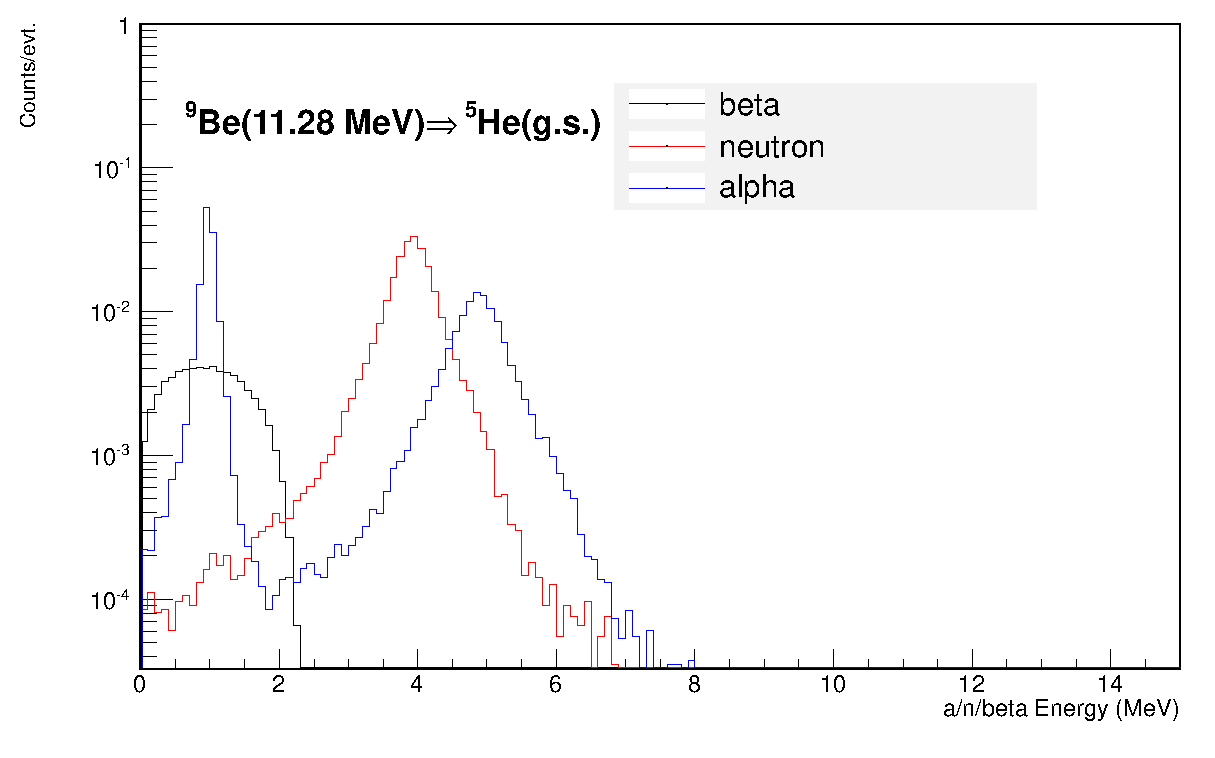
\includegraphics[width=70mm]{a_n_beta_spect_c11.eps} &

      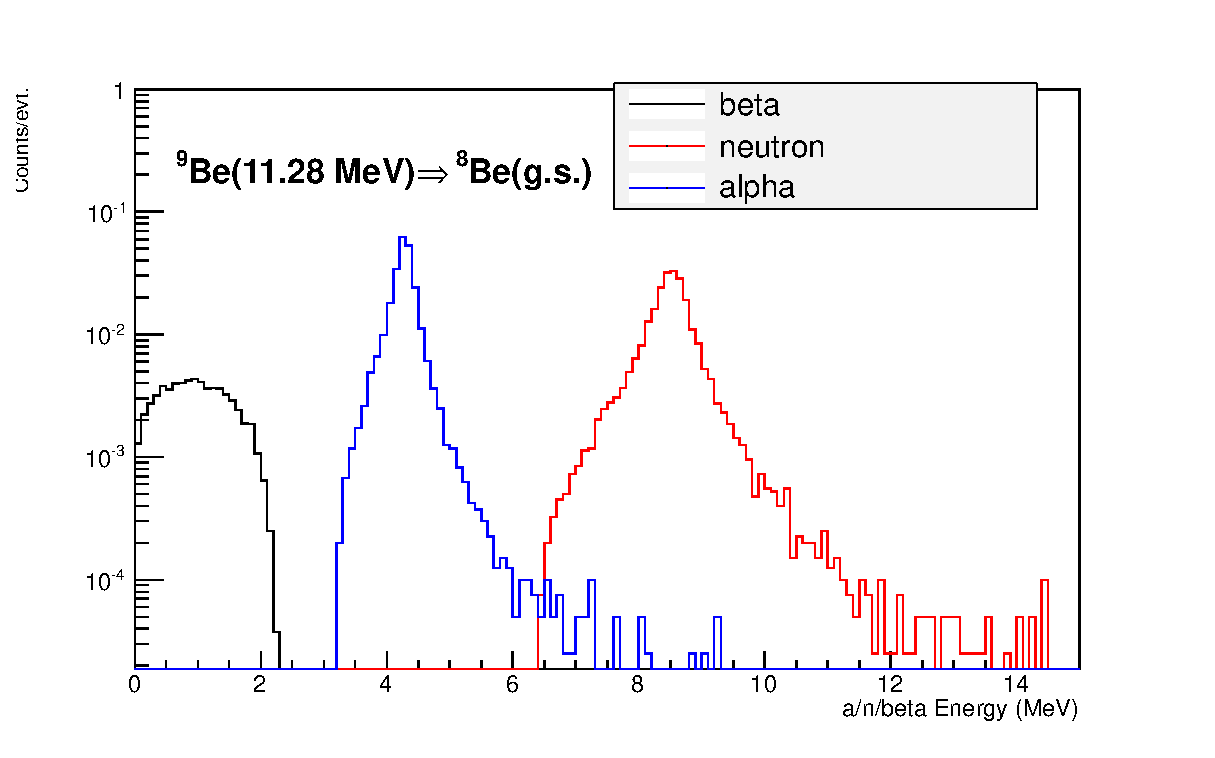
\includegraphics[width=70mm]{a_n_beta_spect_c12.eps} \\

    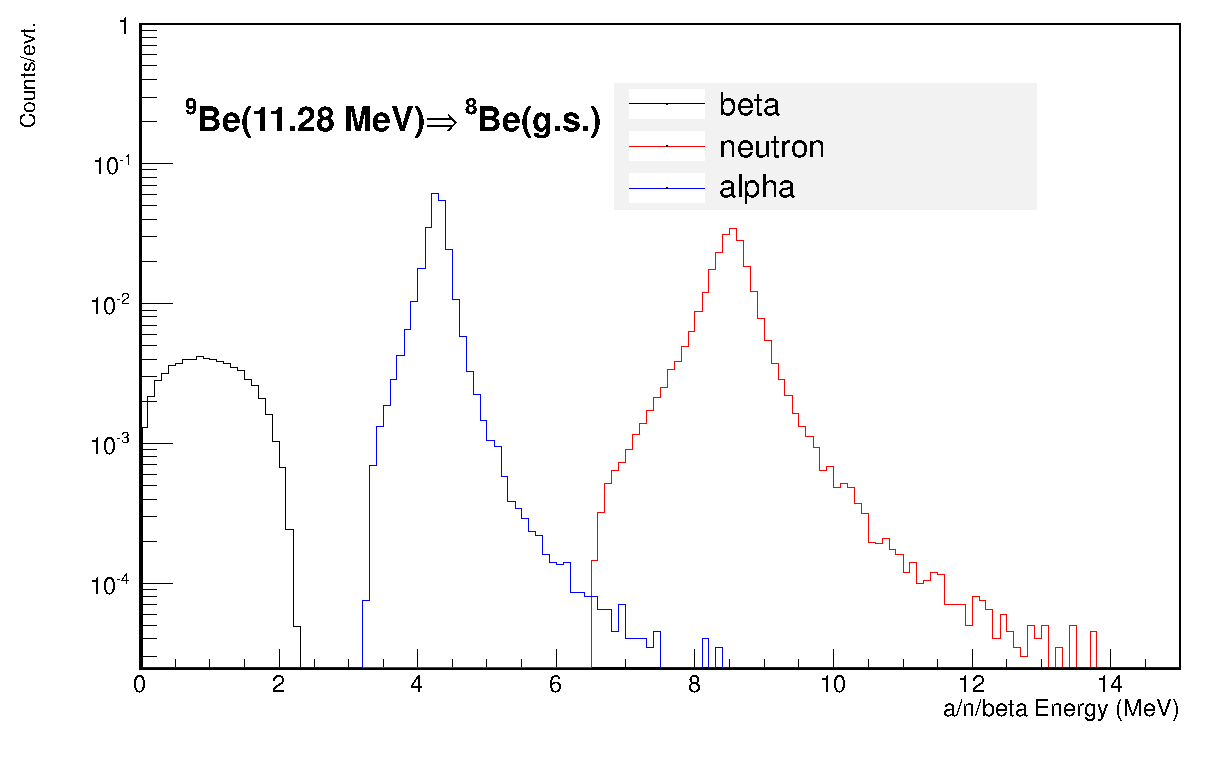
\includegraphics[width=70mm]{a_n_beta_spect_c13.eps} &
   
   
    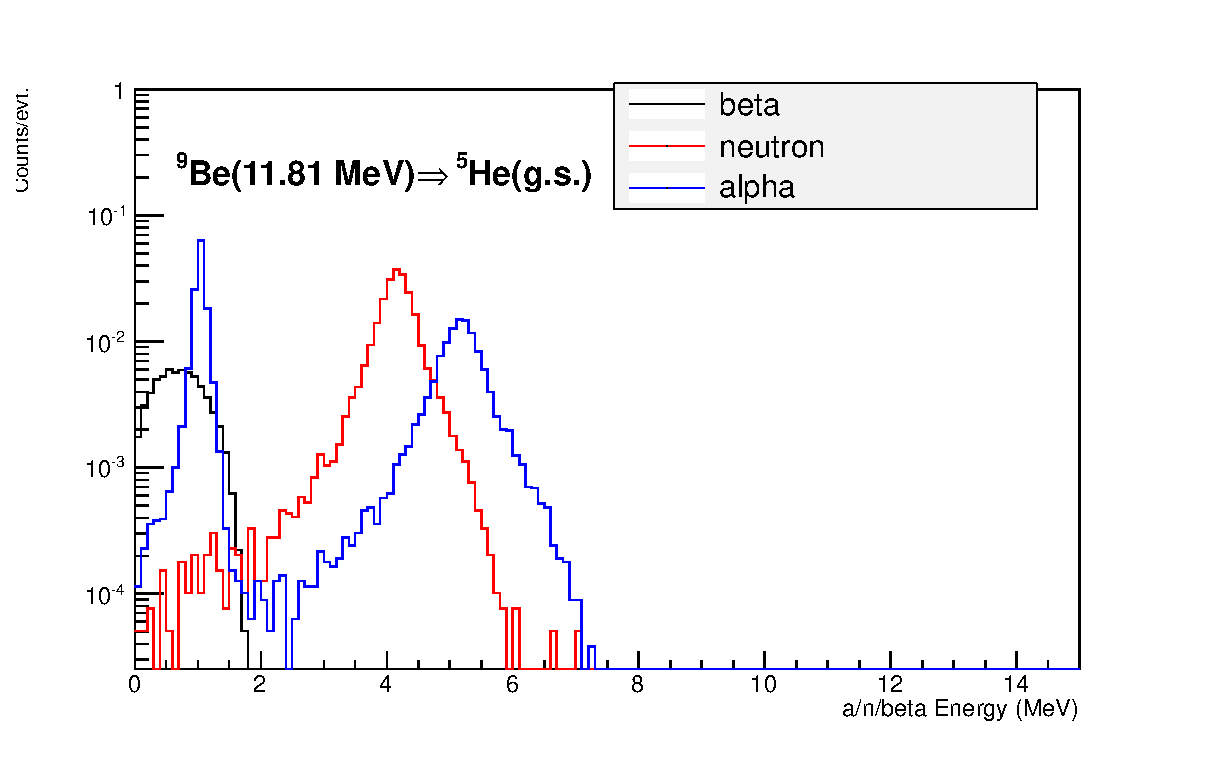
\includegraphics[width=70mm]{a_n_beta_spect_c14.eps} \\

    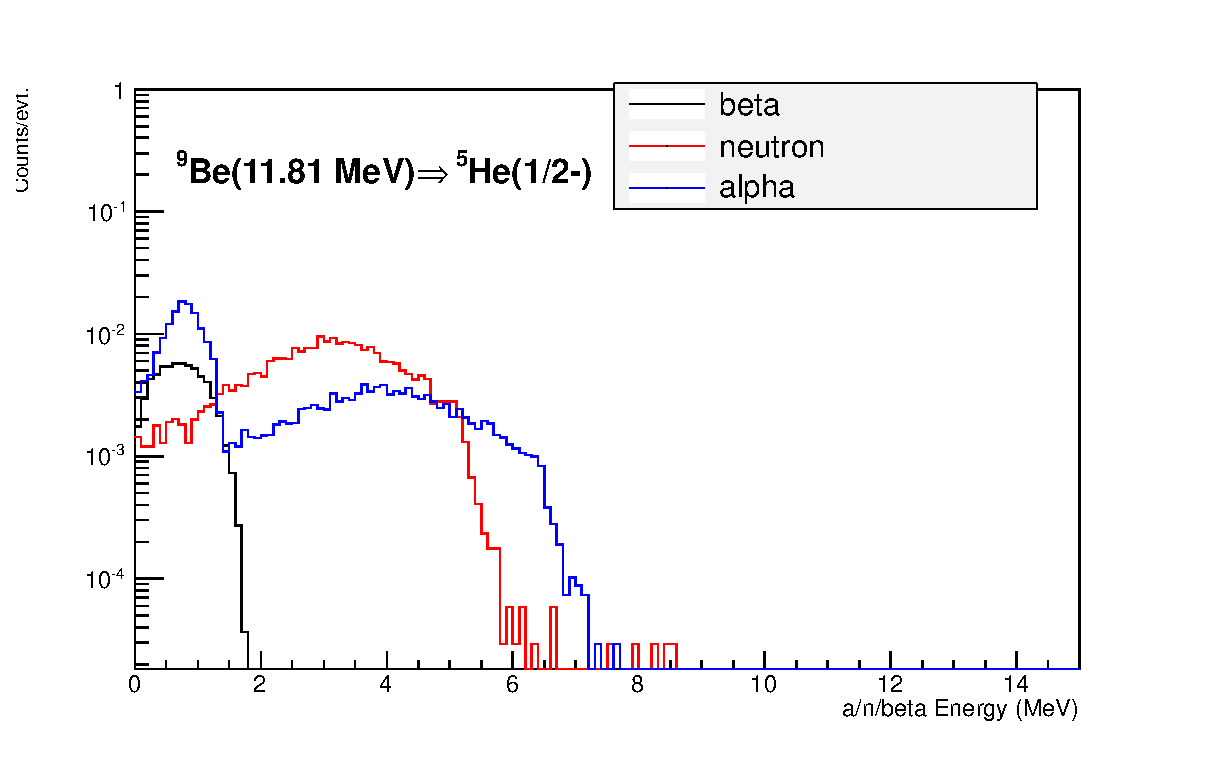
\includegraphics[width=70mm]{a_n_beta_spect_c15.eps}\\
    
    
      \end{tabular}
     \caption{Particle level energy distributions for the decay of the \beNINE 11.28 MeV state.}
    \end{figure}
%%%%%%%%%%%%%%%%%%%%%%%%%%%%%%%%%%%%%%%%%%%%%
%%%%%%%%%%%%%%%%%%%%%%%%%%%%%%%%%%%%%%%%%%%%%
   \begin{figure}[htp]
     \centering
   
  \begin{tabular}{cc}
    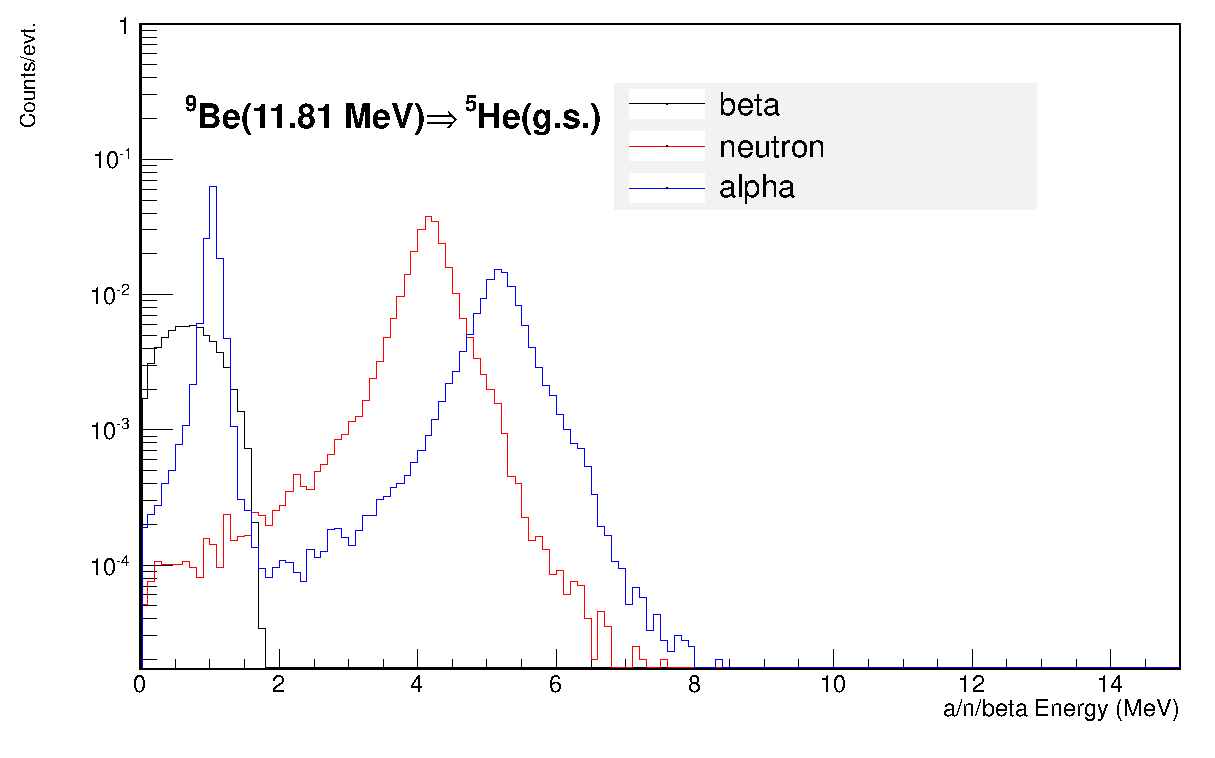
\includegraphics[width=70mm]{a_n_beta_spect_c16.eps}&

    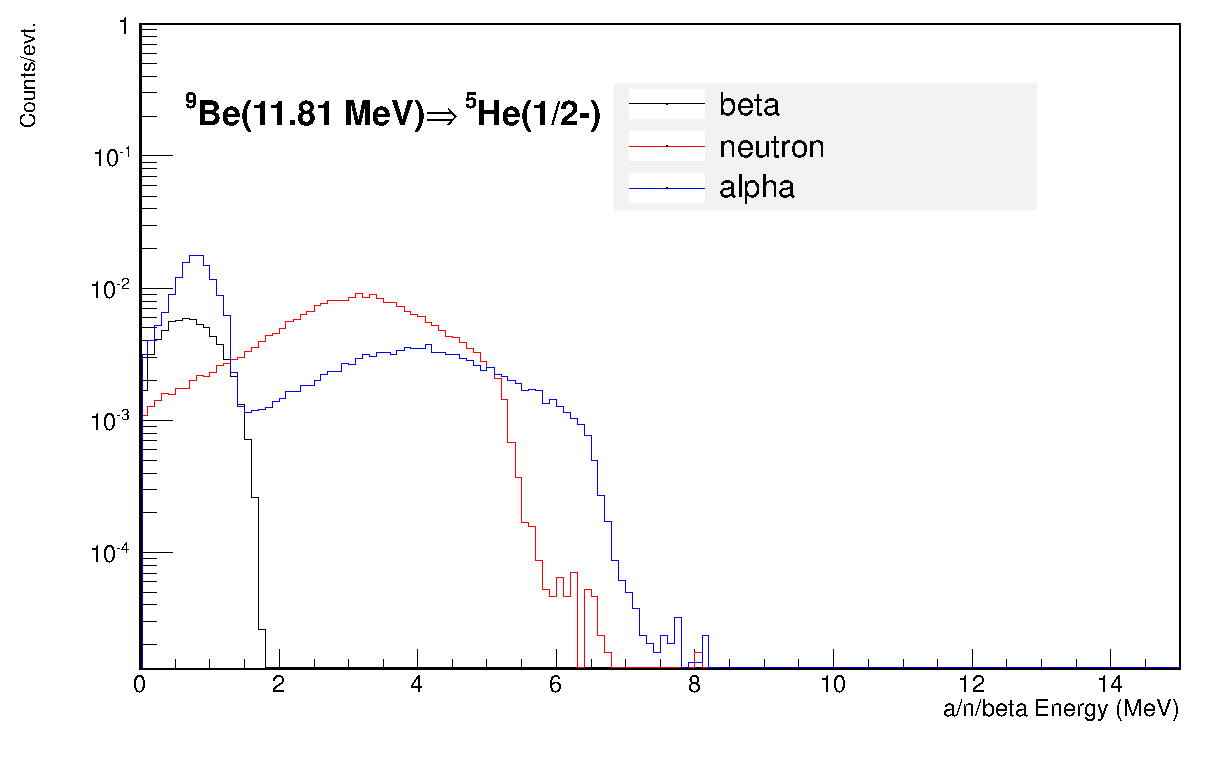
\includegraphics[width=70mm]{a_n_beta_spect_c17.eps}\\
    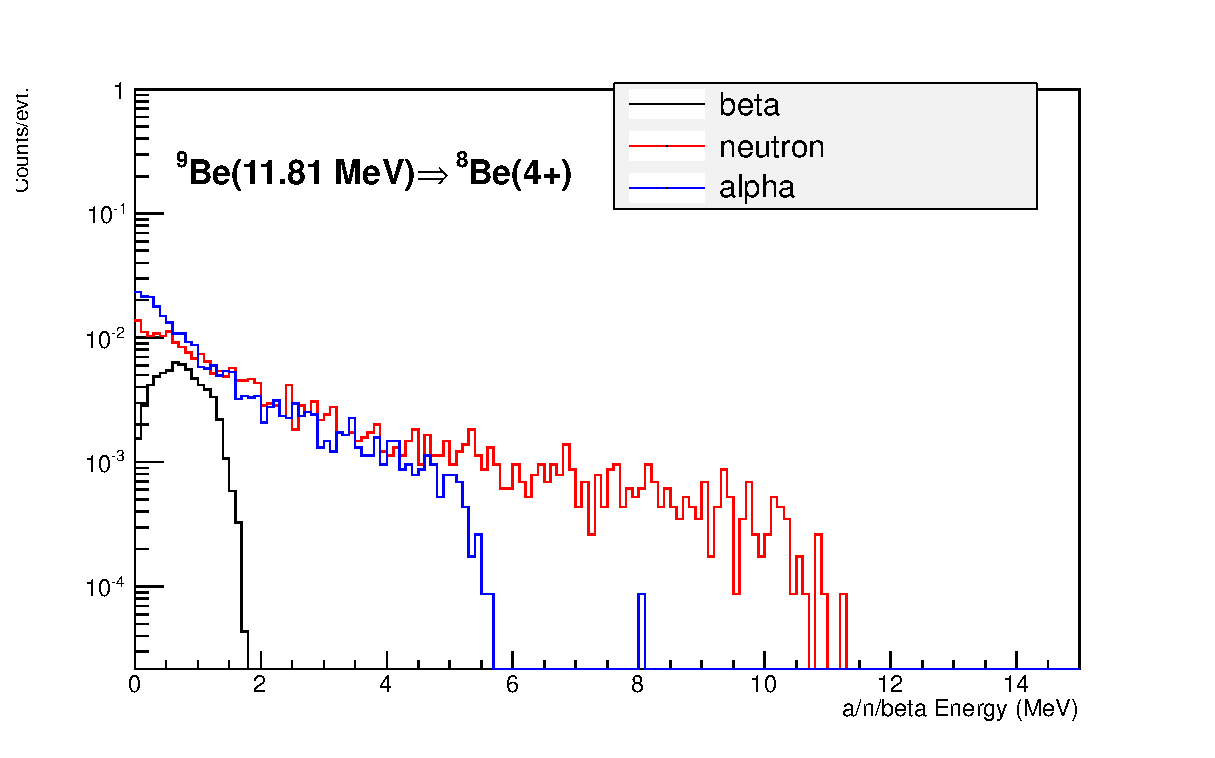
\includegraphics[width=70mm]{a_n_beta_spect_c18.eps}&

    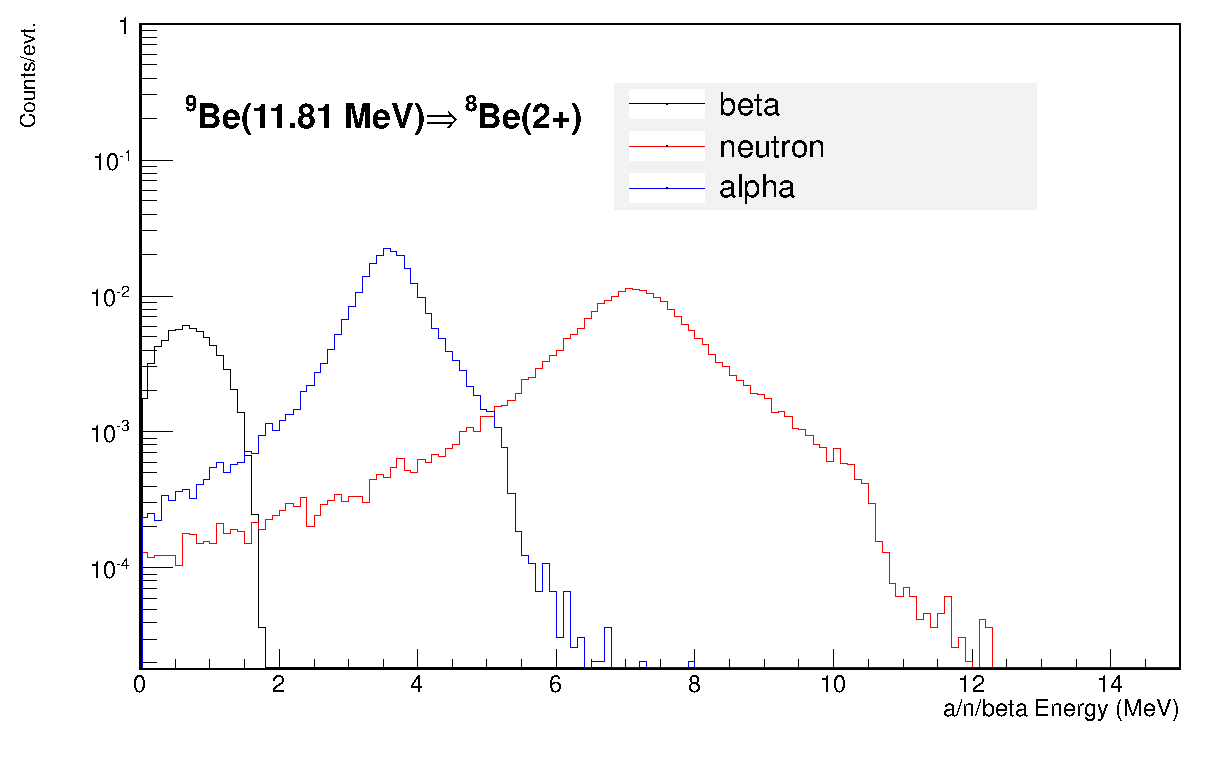
\includegraphics[width=70mm]{a_n_beta_spect_c19.eps}\\
    
    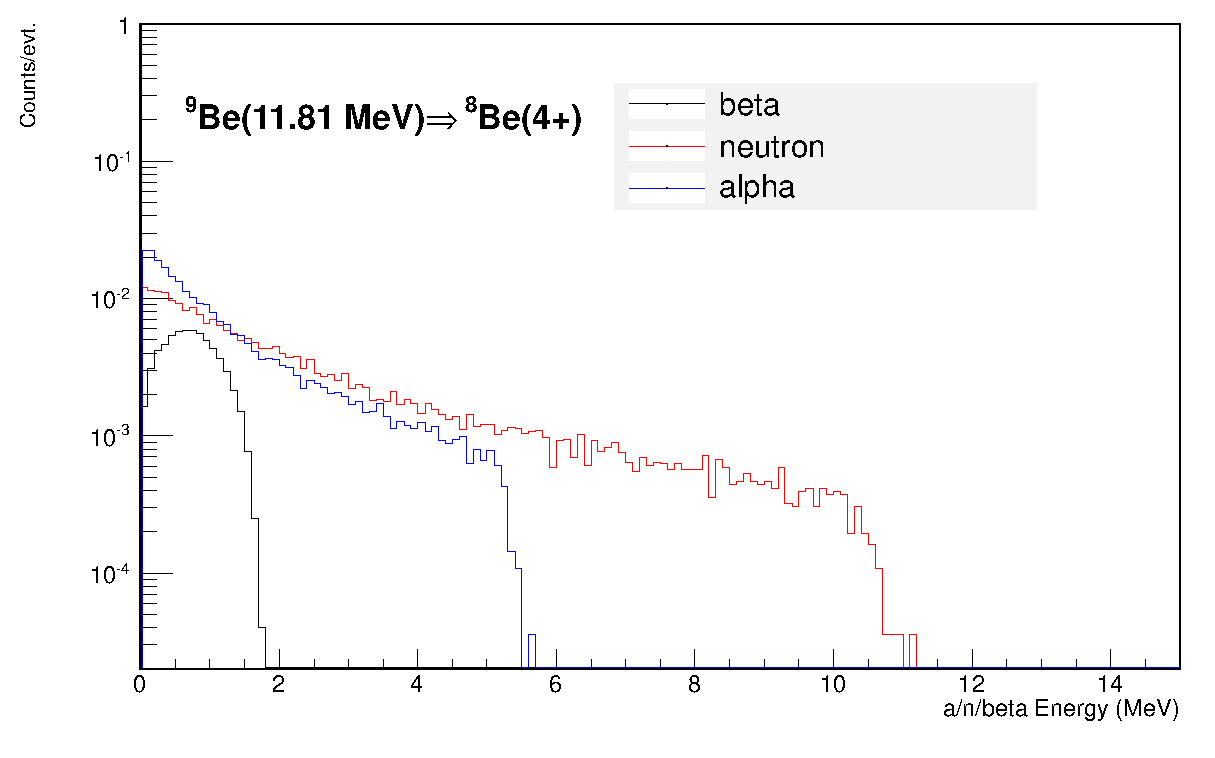
\includegraphics[width=70mm]{a_n_beta_spect_c20.eps}&
   
    \end{tabular}
     \caption{Particle level energy distributions for the decay of the \beNINE 11.81 MeV state.}
    \end{figure}
       
       
       For the particle level results the generator was run with the "one branch" switch illustrated in fig.~\ref{PartDetDiagram},
       in such mode of the generator each branch/subbranch is specifically selected and generated with 100\% probability.
       The output neutron, alpha and beta energies are shown in the figures. The distributions show a clear structure of the energy transformed in each case, 
       visible as a peak broadened by its assigned width.%fig.~\ref{Particle_level_energies}.

       
       We also show the scatter plot of the sum of all the particle energies (alphas, neutrons and betas) as a function 
       of each of the particle's energy, fig.~\ref{histAA}
       
       \begin{figure}[htp]
    \begin{center}
  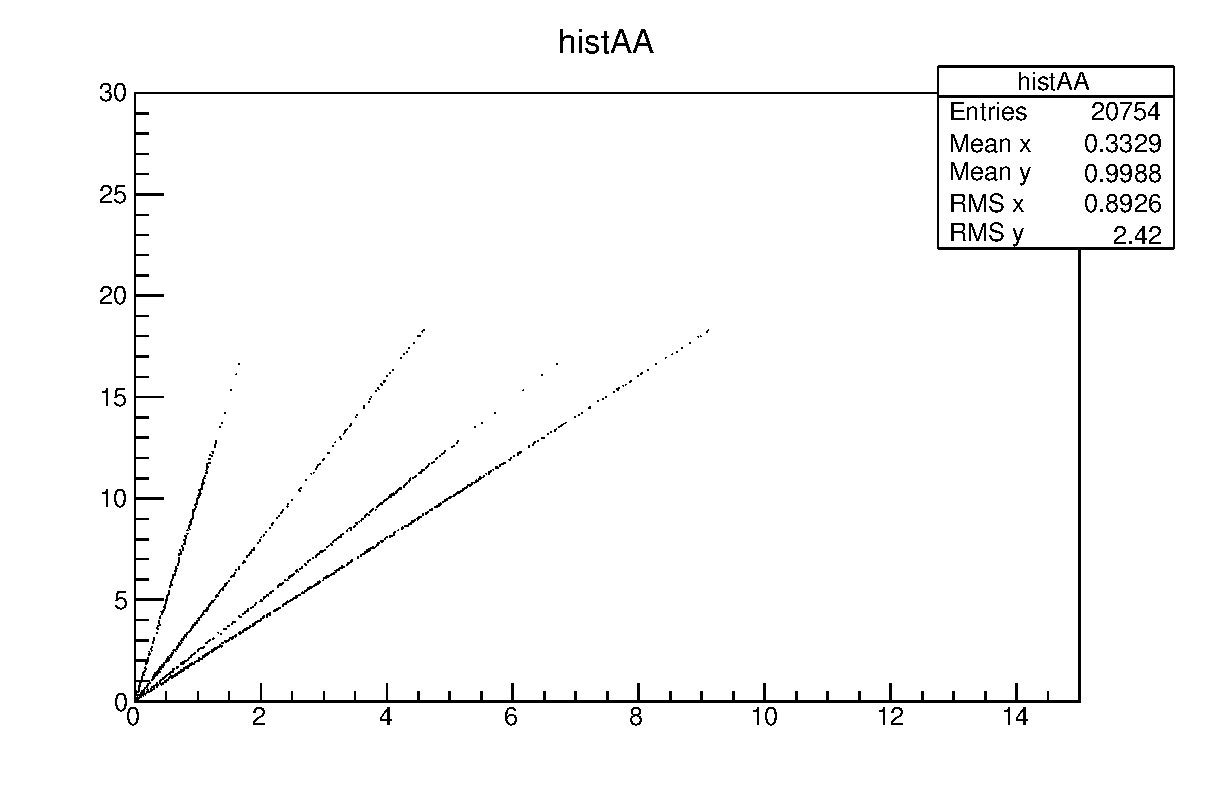
\includegraphics[scale=0.65]{histAA.eps}
   \label{histAA}
    \end{center}
    \caption{ Correlation of the sum of energies of alphas, neutrons or betas vs. the energy of each of them. We should also note that 
    in this plot there is a degenercy of particle energyies; a single point on the vertical axis has three corresponding points on the
    horizontal. This plot was done in line with figure 5 in ~\cite{Prezado200543}.}
 \end{figure}

   


\subsection{Detector Level}

       The output of the generator is the raw energy deposited in the detector, as such refered to as detector level. To select \liNINE events we use the 
       cuts commonly used by reactor-based experiments for their cosmogenics selection. A \liNINE candidate is selected based on a 
       coincidence between a prompt and a delayed event. The prompt event is defined as an event that has energy; $ 0.7 < E_{prompt} < 12.0$ MeV, while the 
       delayed having energy; $ 6.0 < E_{delayed} < 12.0$ MeV. The coincidence has to lie within a time window of $2 \mu s < \Delta T_{prompt-delayed} < 100 \mu s $
       with no triggers in the; 
       100 $\mu$s preceeding the prompt and 400 $\mu$s following the prompt.
       
       
       In fig. ~\ref{MC_full} is the output of the Double Chooz simulation of the generator after weighting each of the branches by its appropiate 
       ratio. The figure shows the prompt energy distributions for the prompt-delayed coincidence. It is worth noting that the 
       prompt energy used here is the calibrated energy of the Double Chooz detector.
       

       \subsection*{\it Branching uncertainties}

      The branching ratios also have associated uncertainties. In order to determine the sub-branch with the most branching ratio uncertainty, we 
      evaluate the errors for such sub-branches. In fig.~\ref{BRUncert_1} are the combined uncertainties
      of all the different combination of allowed branches and sub-branches for the cases of fluctuating betas and/or heavies.
      
      Also, in fig~\ref{BRUncert_2}
      are the errors for the case of only the heavies' branching ratios being varied. As evidenced by the bottom plot, no conclusion can be made yet 
      of the most uncertain branch.
           
       \begin{figure}[htp]
 \begin{center}
  
  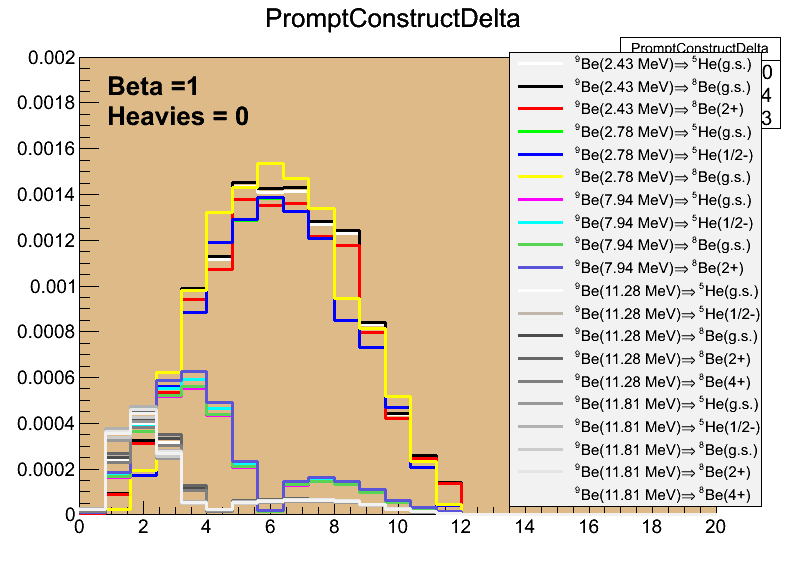
\includegraphics[scale=0.45]{canvas_1_0.png}
  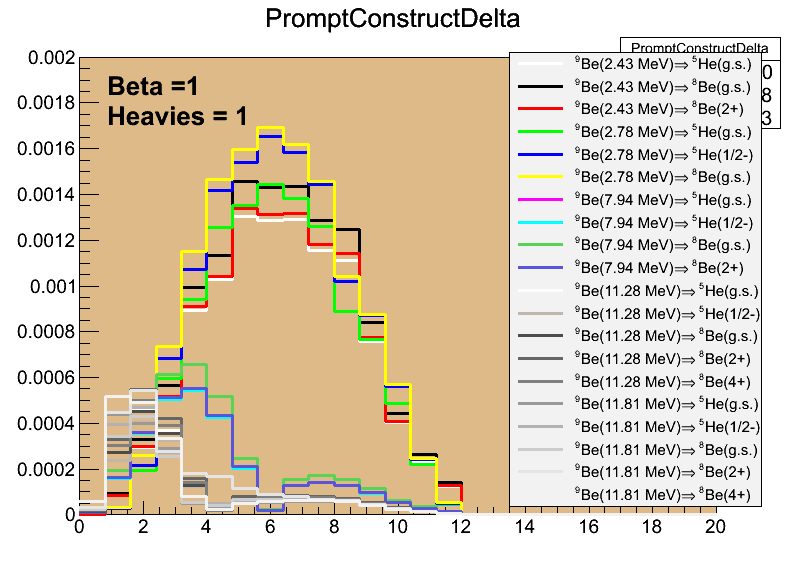
\includegraphics[scale=0.45]{canvas_1_1.png}
   \label{BRUncert_1}
    \end{center}
    \caption{ (From top to bottom) The width of the uncertainties for the different branch and sub-branch decay routes for the case of fluctuating
    the beta decay branching ratios but not the heavies; for the case of fluctuating both the beta decay branching ratios and also the heavies}
    \end{figure}
    
  
    \begin{figure}[htp]
 \begin{center}
  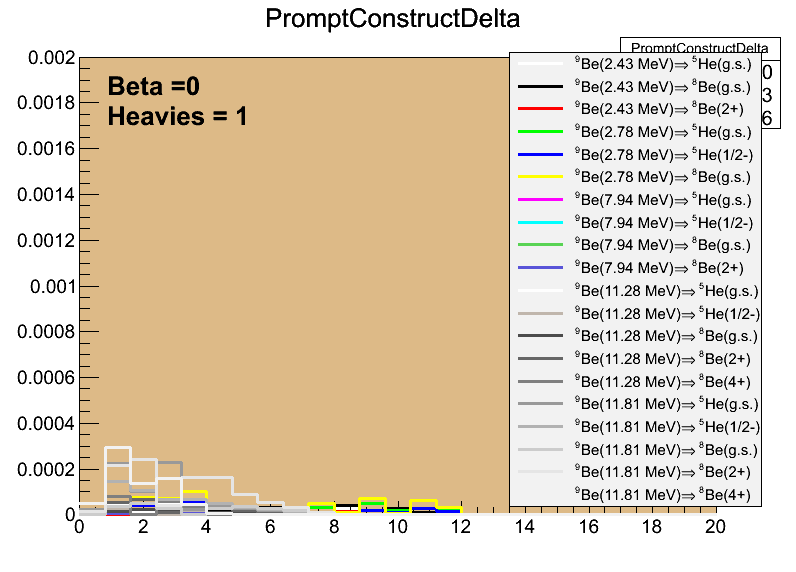
\includegraphics[scale=0.45]{canvas_0_1.png}
   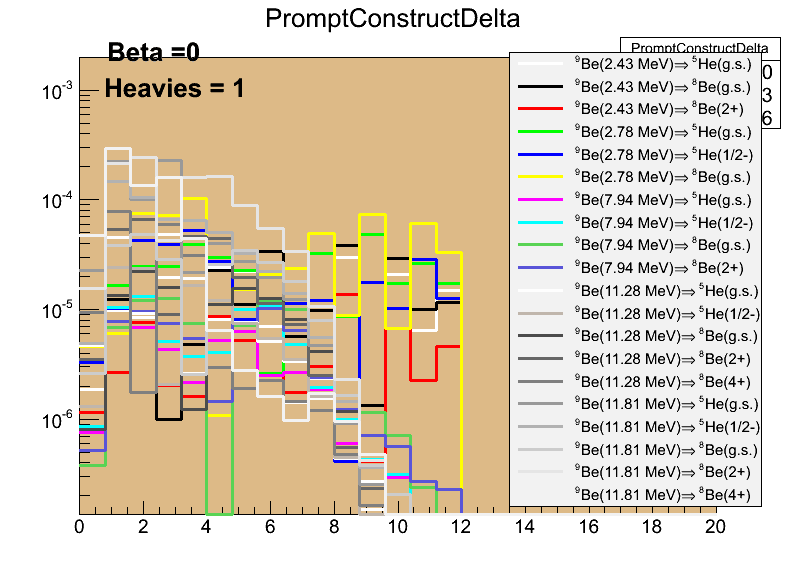
\includegraphics[scale=0.45]{log_canvas.png}
   \label{BRUncert_2}
    \end{center}
    \caption{ (Above) Same as previous figure but for the case of not fluctuating the betas and doing it for the heavies. (Bottom) On a logarithmic
    scale.}
    \end{figure}
      
      
      .........
      .....
      ..

       
       
       \begin{figure}[htp]
 \begin{center}
  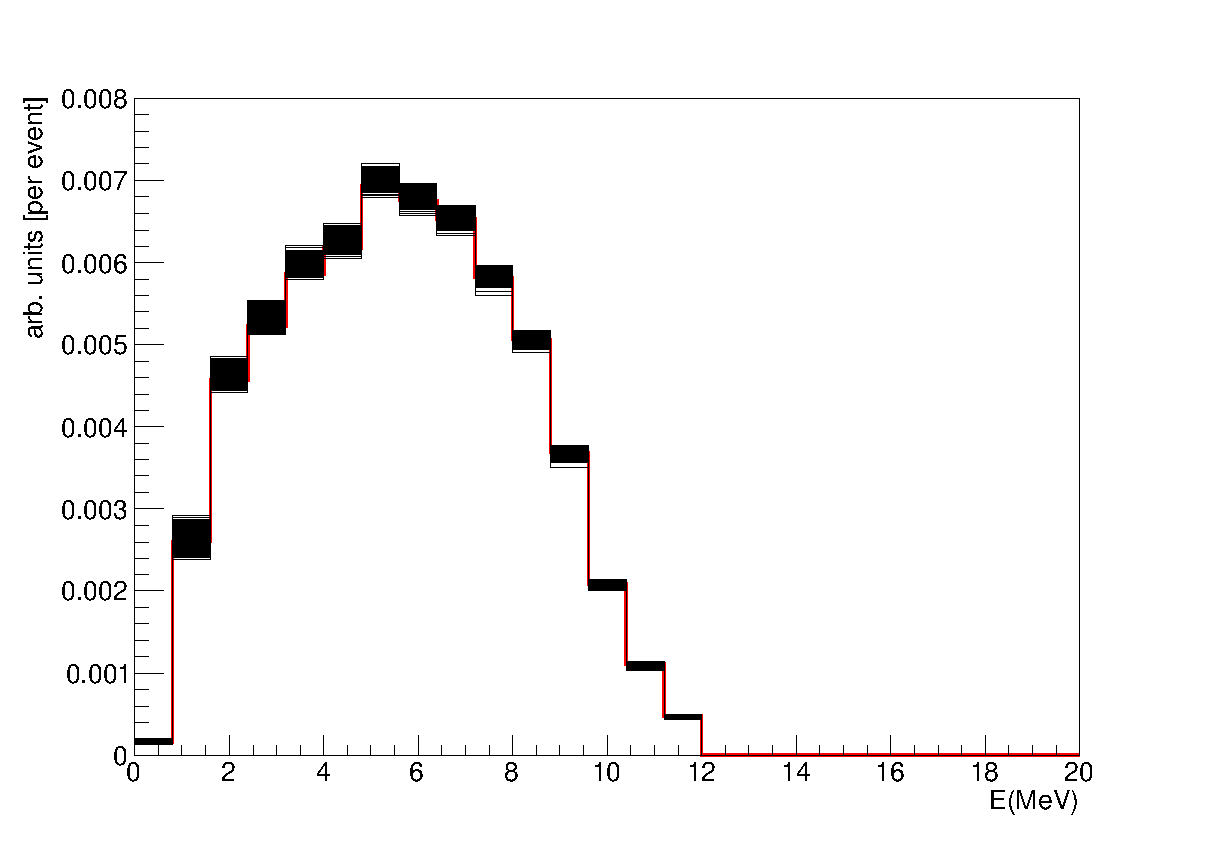
\includegraphics[scale=0.65]{MC_full_withErrors.eps}
  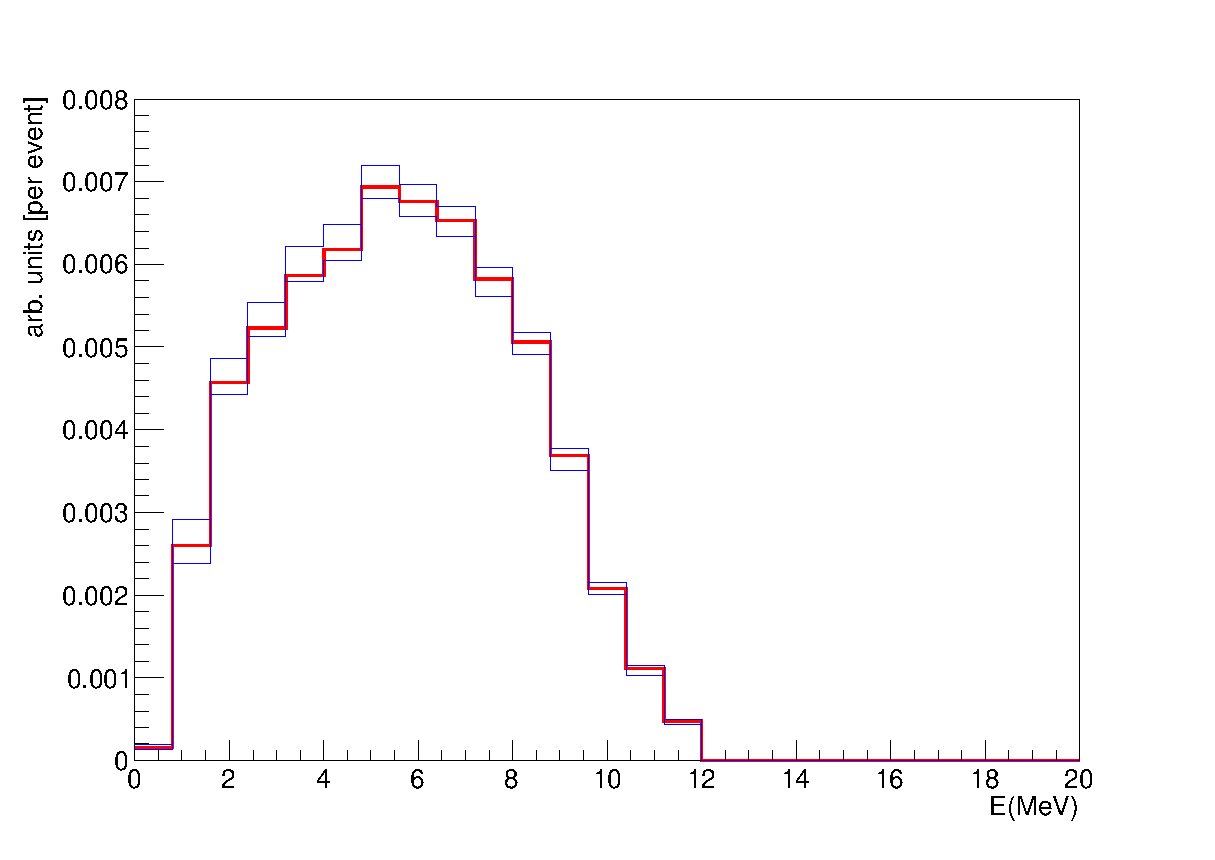
\includegraphics[scale=0.65]{MC_full.eps}
   \label{MC_full}
    \end{center}
    \caption{ (Above) The prompt spectra for the \liNINE simulation output after adding up all the branches with their weights. The Fluctuations of the branching ratios 
    are also shown as a way to estimate the branching ration uncertainties. (Below) The extracted branching uncertainties forming an " envelope". }
 \end{figure}

       
%\begin{figure}[htp]

 % \centering

  

%  \begin{tabular}{cc}

%    % Requires \usepackage{graphicx}

 %   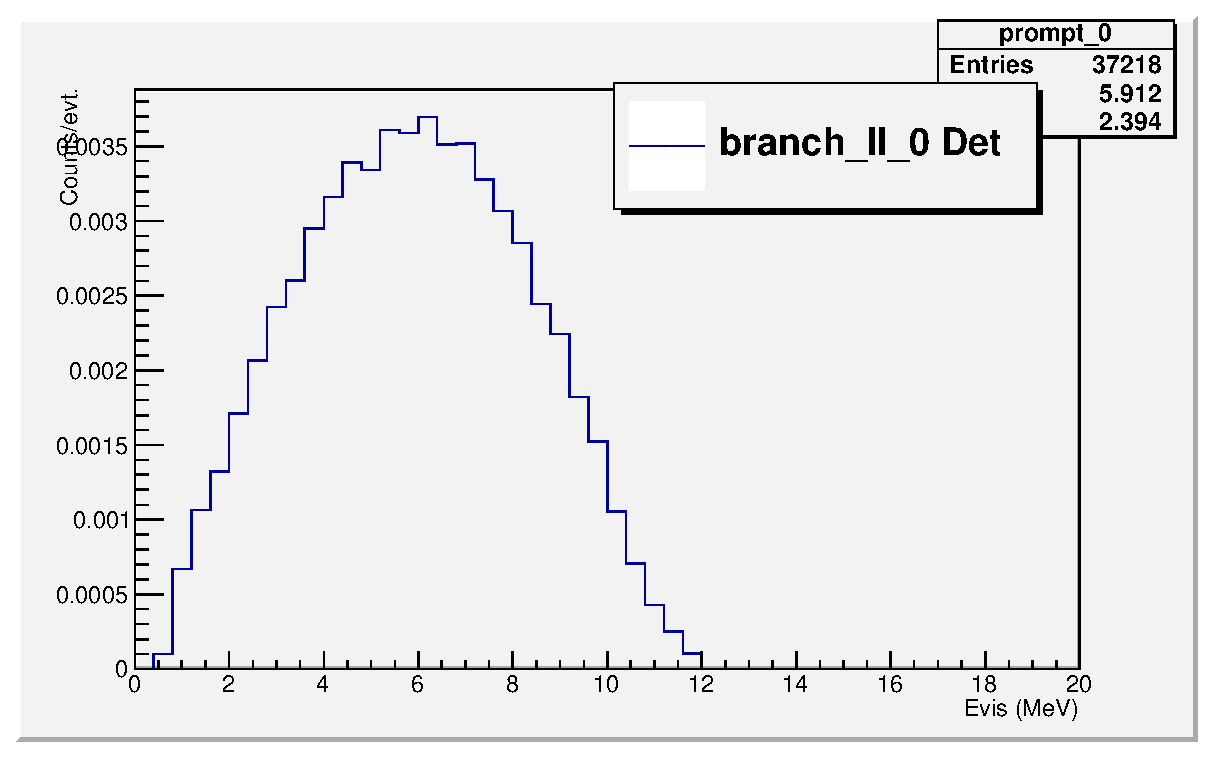
\includegraphics[width=60mm]{MC_Li_10.eps}&

  %  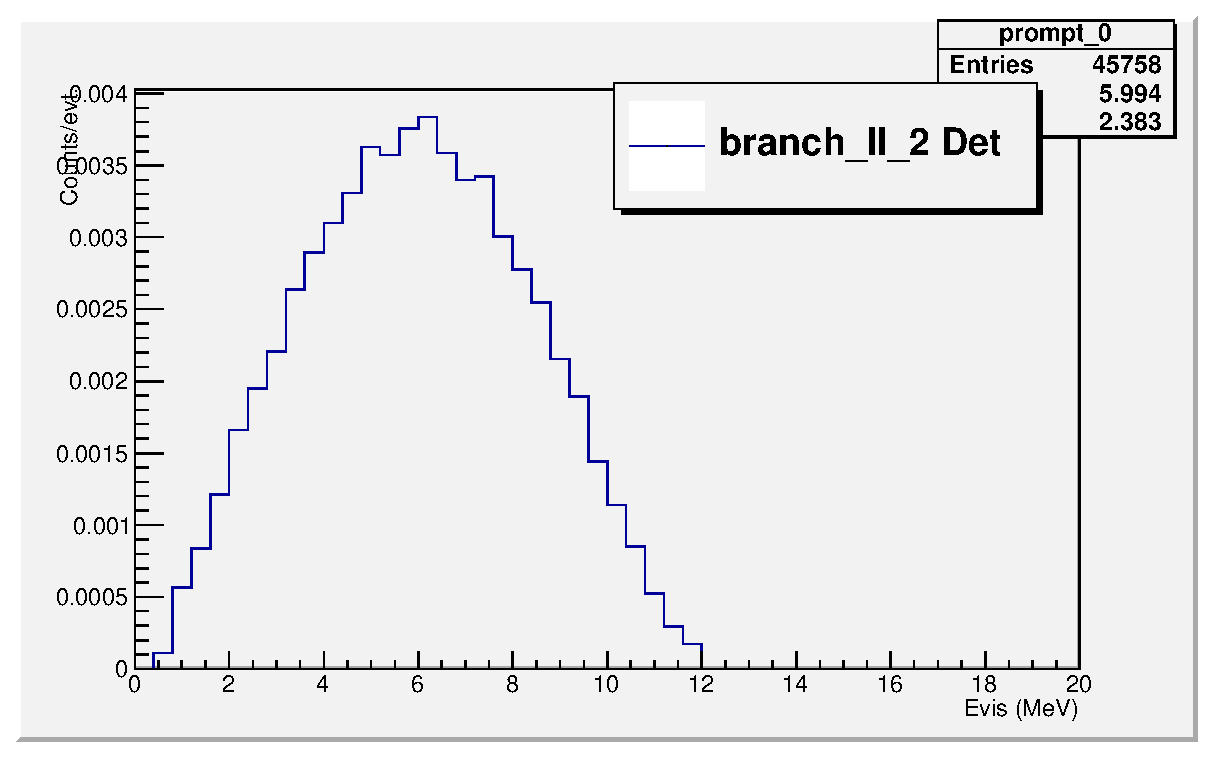
\includegraphics[width=60mm]{MC_Li_12.eps}\\

   % 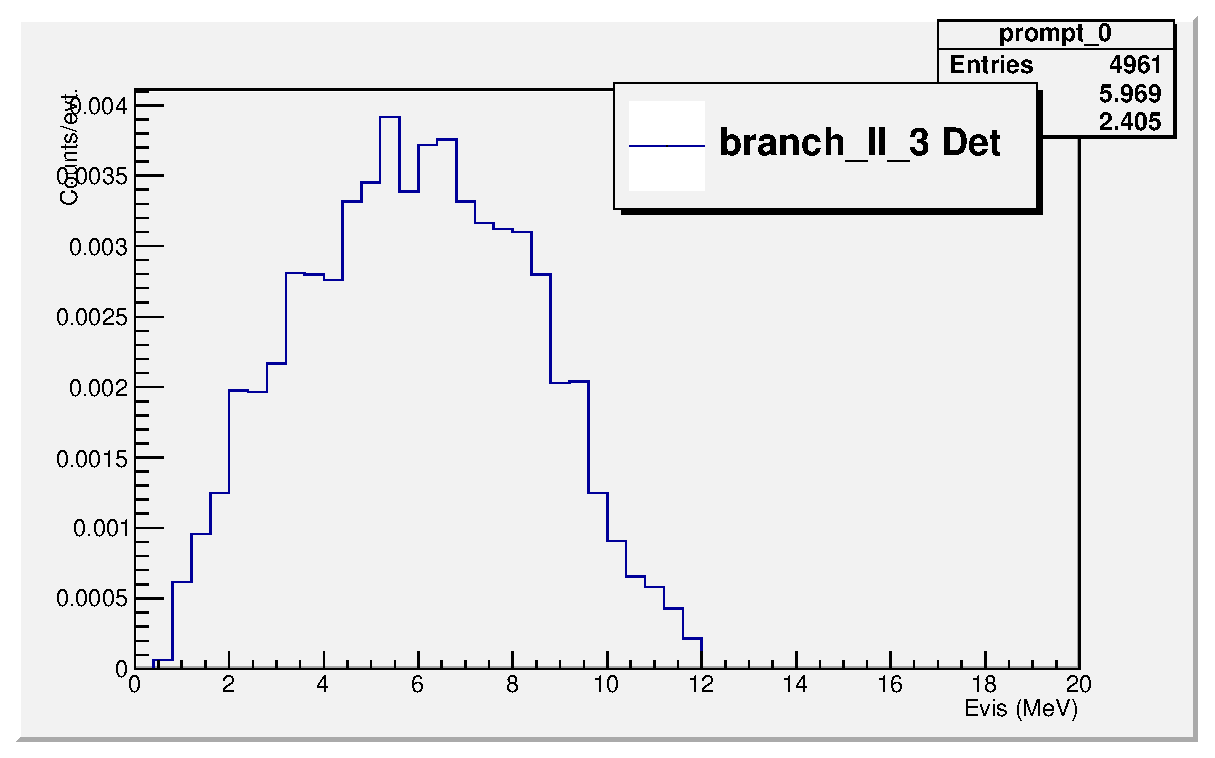
\includegraphics[width=60mm]{MC_Li_13.eps}&

    %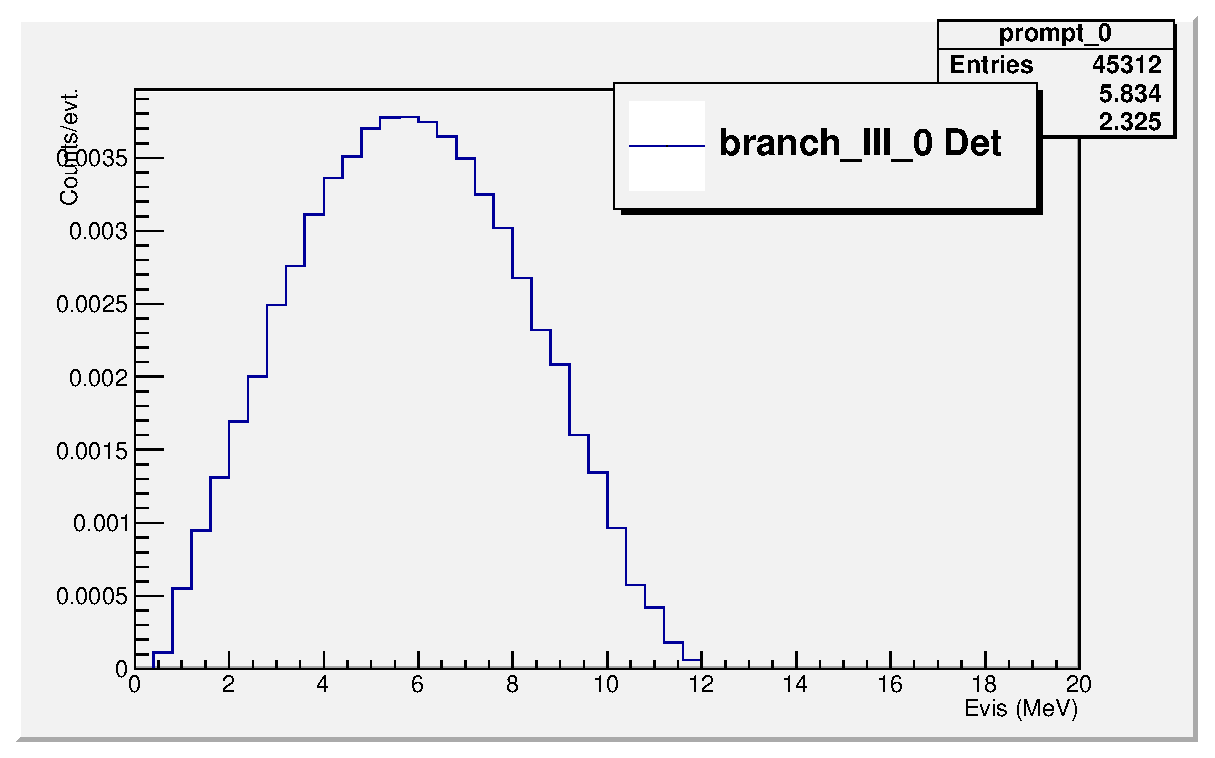
\includegraphics[width=60mm]{MC_Li_20.eps}\\

    %  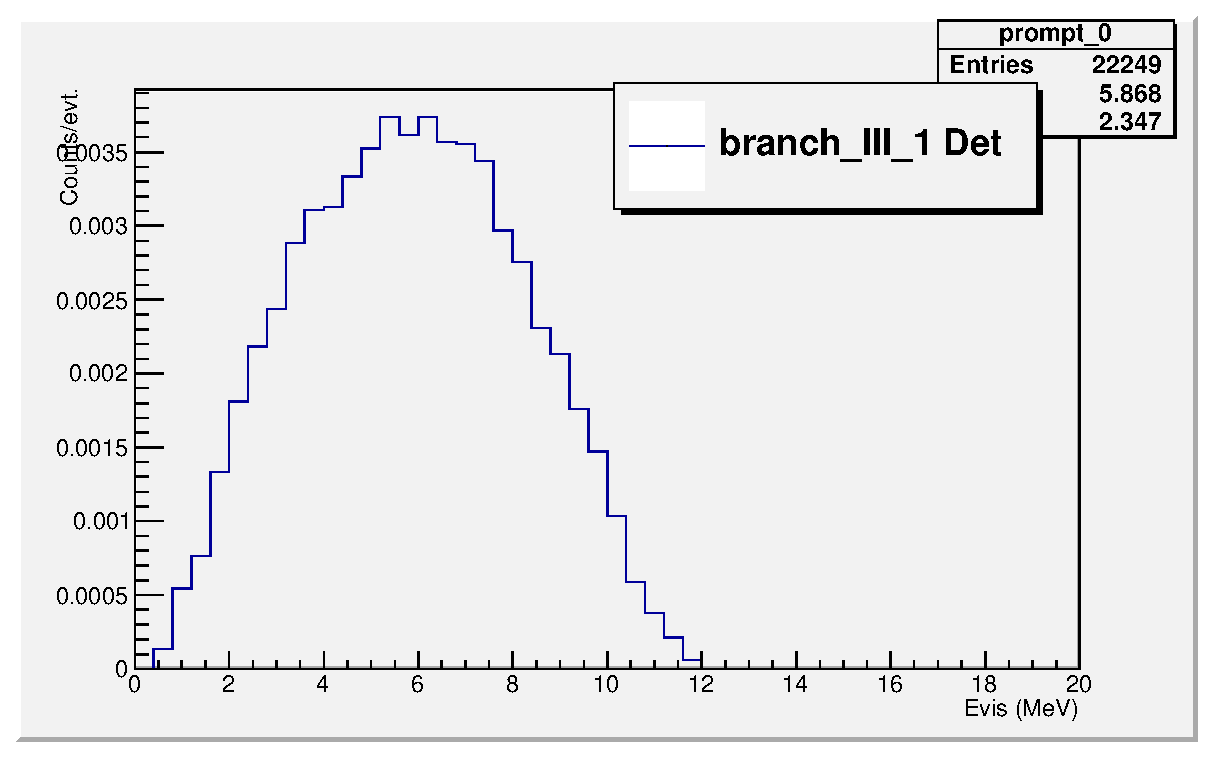
\includegraphics[width=60mm]{MC_Li_21.eps}&

%    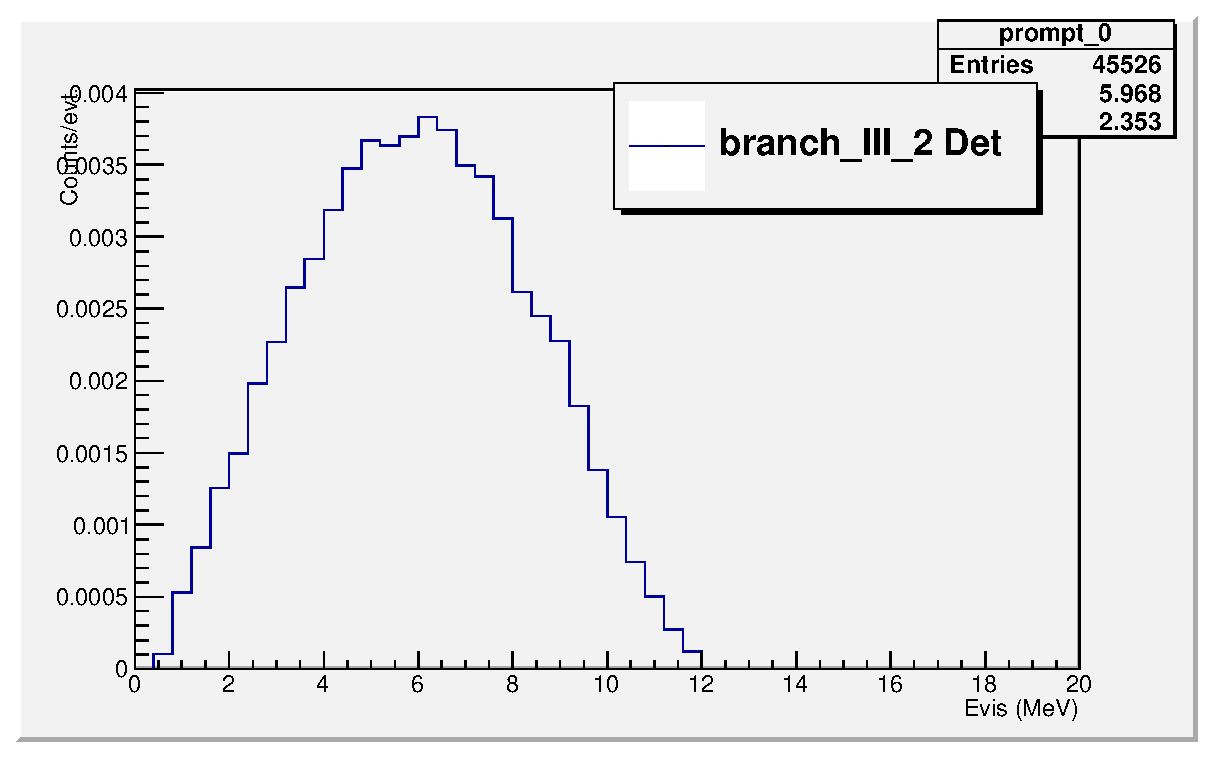
\includegraphics[width=60mm]{MC_Li_22.eps}\\
   
 % \end{tabular}
%\label{figur2}\caption{ Detector level energy distributions.}
%\end{figure}



       


\section{Conclusions}
\label{section3}

.................................................................
.................................................................
.................................................................
.................................................................
.................................................................
...................
.............

...........
..

\acknowledgments

       We acknowledge the support of the Pays de La Loire grant XXXX and MIT grant XXXX. M. E.  would
       like to specifically thank Dr. Muriel Fallot and the ERDRE team at the EMN/IN2P3/CNRS funded laboratory SUBATECH in France 
       for their hospitality and support.


\bibliography{mybib}{}
\bibliographystyle{plain}

\end{document}
